\documentclass[12pt]{article}
\usepackage[a4paper, total={6in, 8in}]{geometry}
\usepackage{amsfonts}
\usepackage{amsmath,amssymb,trimclip,adjustbox}
\usepackage{breqn}
\usepackage{hyperref}
\usepackage{tabularray}
\usepackage[dvipsnames]{xcolor} 
\usepackage{polski}
\usepackage[utf8]{inputenc}

\newcommand{\suminfty}[1]{\sum\limits_{n = #1}^{\infty}}
\newcommand{\dpartial}[2]{\frac{\partial #1}{\partial #2}}
\newcommand{\limn}{\lim_{n \to \infty}}


\setlength{\parindent}{0pt}
\setlength{\textheight}{680pt}
\setlength{\oddsidemargin}{-5pt}
\setlength{\textwidth}{480pt}

\everymath{\displaystyle}

\author{(nieoficjalny) Skrypt wykładu Krzysztofa Michalika}
\title{Wykład - Analiza matematyczna II}

\begin{document}
\maketitle
\tableofcontents

\subsection{Mały wstęp}

Skrypt jest w większości przepisywany ze zdjęć zrobionych w wordzie z dysku ale w przypadku jakichś braków wykorzystywana jest
prezka dr. Michalika. 

W skrypcie mogą pojawić się błędy stąd najlepiej przed nauką pobrać z dysku najbardziej aktualną wersję
zamieszczoną w folderze 

Semestr II $->$ Analiza Matematyczna2 $->$ Michalik wykłady $->$ Skrypt\_Wykład.pdf.

Data którą można zobaczyć na samym górze jest \textbf{datą ostatniej aktualizacji skryptu}.

Wszelkie uwagi, błędy (na pewno jakieś są) można pisać priv na discordzie : 

\textbf{Tomasz Strzelba\#1454}

Miłej nauki!

\section{Całki niewłaściwe I rodzaju}

Ustalamy liczbę $a \in \mathbb{R}$. Niech $f$ będzie funkcją całkowalną na każdym przedziale \linebreak w postaci $[a, T]$
gdzie $T > a$. Definiujemy \underline{całkę niewłaściwą pierwszego rodzaju} z $f$ na półprostej $[a, \infty]$ jako

$$ \int\limits_{a}^{\infty} f(x) \,dx = \lim_{T \to \infty} \int\limits_{a}^{T} f(x) \,dx \ \text{,  gdy granica po prawej stronie istnieje} $$

Analogicznie, gdy $f$ jest całkowalna na każdym przedziale postaci $[T, b]$, gdzie $T < b$. Definiujemy całkę niewłaściwą
pierwszego rodzaju z $f$ na półprostej [$-\infty$, b] jako

$$ \int\limits_{-\infty}^{b} f(x) \,dx = \lim_{T \to -\infty} \int\limits_{T}^{b} f(x) \,dx \ \text{,  gdy granica po prawej stronie istnieje} $$\\

Terminologia dotycząca takich całek jest taka, jak dla ciągów. Są 3 przypadki :

\begin{enumerate}
    \item Granica z prawej strony jest liczbą. Wtedy mówimy, że całka jest \underline{zbieżna}.
    \item Granica z prawej strony jest równa $\infty$ lub $-\infty$. Wtedy mówimy, że całka jest \underline{rozbieżna} (odpowiednio do $\infty$ lub $-\infty$).
    \item Granica z prawej strony nie istnieje. Wtedy mówimy, że całka jest \underline{rozbieżna}.
\end{enumerate}

Analogicznie dla $ \int\limits_{\infty}^{b} f(x)\,dx $

Przykłady :

$$ \int\limits_{0}^{\infty} \sin x \,dx = \lim_{T \to \infty} \int\limits_{0}^{T} \sin x \,dx = 
\lim_{T \to \infty} [-\cos x]_0^T = \lim_{T \to \infty} (-\cos T - (- \cos 0)) = \lim_{T \to \infty} (1 - \cos T) $$

Granica ta nie istnieje więc całka jest rozbieżna. \\

$$ \int\limits_{-\infty}^{0} 2^x \,dx = \lim_{T \to -\infty} \int\limits_{T}^{0} 2^x \,dx = 
\lim_{T \to -\infty} \left[ \frac{2^x}{\ln 2} \right]_T^0 = \lim_{T \to -\infty} 
\left( \frac{1}{\ln 2} - \frac{2^T}{\ln 2} \right) = \frac{1}{\ln 2} $$

Całka jest zbieżna do $ \frac{1}{\ln 2} $. \\

Pozostaje przypadek $ p = 1 $. Wtedy

$$ \int \frac{1}{x} \,dx = \ln |x| + C, \ \
\int\limits_{a}^{T} \frac{1}{x} \,dx = [\ln |x|]_a^T = \ln |T| - \ln |a|, \ \
\int\limits_{a}^{\infty} \frac{1}{x} \,dx = \lim_{T \to \infty} (\ln |T| - \ln |a|) = \infty $$

Udowodniliśmy zatem ważny wynik \\

\textbf{Twierdzenie} 

Gdy $ a > 0 $ to całka $ \int\limits_{a}^{\infty} \frac{1}{x^p} \,dx $
jest skończona dla $ p > 1 $ oraz nieskończona dla $ p \leq 1 $.

Podobnie można łatwo pokazać poniższy wynik \\

\textbf{Twierdzenie}

Gdy $ a \in \mathbb{R} $ i $ A > 0 $ to całka $ \int\limits_{a}^{\infty} A^x \,dx $
jest skończona dla $ 0 < A < 1 $ oraz nieskończona \linebreak dla $ A \geq 1 $ \\

Gdy $ \int f(x) \,dx = F(x) + C $ \ to

$$ \int\limits_{-\infty}^{\infty} f(x) \, dx = \lim_{T \to \infty} F(T) - \lim_{S \to \infty} F(S) $$

przy czym przynajmniej jedna z granic z prawej strony nie istnieje lub zachodzi przypadek 
$ \infty - \infty $ to $ \int\limits_{-\infty}^{\infty} f(x) \,dx $ jest rozbieżna, a w pozostałych
przypadkach całka ma wartość wynikającą z arytmetyki granic. \\

W przypadku kiedy całki nie da się obliczyć w sposób dokładny można to zrobić w sposób przybliżony, pod warunkiem
, że wiemy, że jest zbieżna.

Kryteria zbieżności to twierdzenia opisujące warunki dostateczne zbieżności lub rozbieżności danej klasy
całek. Najczęściej mają postać implikacji ale NIE równoważności. \\

Oznacza to zwykle własności postaci

\quad warunek zachodzi $ \Rightarrow $ całka jest zbieżna/rozbieżna

\quad warunek nie zachodzi $ \Rightarrow $ nic nie wiemy o zbieżności/rozbieżności całki

\subsection*{Popularne kryteria zbieżności całek z $\infty$}

0. Warunek konieczny zbieżności całki

Jeżeli całka $ \int\limits_{a}^{\infty} f(x) \,dx $ jest zbieżna to 
$ \lim\limits_{x \to \infty} f(x) $ jest równa 0 lub nie istnieje. \\

Transpozycja twierdzenia daje następujący wynik:

Jeżeli $ \lim\limits_{x \to \infty} f(x) $ istnieje i jest różna od 0 to całka 
$ \int\limits_{a}^{\infty} f(x) \, dx $ nie jest zbieżna, przy czym

\begin{itemize}
    \item gdy $ \lim\limits_{x \to \infty} f(x) > 0 $ to $ \int\limits_{a}^{\infty} f(x) \,dx = \infty $,
    \item gdy $ \lim\limits_{x \to \infty} f(x) < 0 $ to $ \int\limits_{a}^{\infty} f(x) \,dx = -\infty $,
\end{itemize}

\textbf{Uwaga. Warunek konieczny to tylko implikacja!}

Jeżeli $ \lim_{x \to \infty} f(x) $ jest równa 0 lub nie istnieje to jeszcze \textbf{NIC NIE WIEMY} o całce,

Na przykład całki $ \int\limits_{a}^{\infty} \frac{1}{x^p} \,dx, \ a > 0 $, mają
$ \lim_{x \to \infty} \frac{1}{x^p} = 0 $ dla wszystkich $ p > 0 $ ale niektóre z tych całek są zbieżne,
a niektóre rozbieżne \\

\subsection*{Ważna klasa całek - całki z funkcji nieujemnych}

$$ \int\limits_{a}^{\infty} f(x) \,dx, \ f \geq 0 $$

Wtedy $ \int\limits_{a}^{T} f(x) \, dx = F(T) - F(a) $ jest funkcją niemalejącą zmiennej T zatem całka
$ \int\limits_{a}^{\infty} f(x) \, dx = \lim_{T \to \infty} \int\limits_{a}^{T} f(x) \,dx $
zawsze istnieje. Może być to liczba lub $\infty$.

Zatem brak zbieżności takich całek oznacza rozbieżność do $\infty$. \\

Dla całek z funkcji nieujemnych mamy dwa kolejne kryteria zbieżności.

\begin{enumerate}
    \item Kryterium porównawcze
    \item Kryterium ilorazowe
\end{enumerate}


\subsection*{Twierdzenie(kryterium porównawcze)}
\addcontentsline{toc}{subsection}{Twierdzenie(kryterium porównawcze)}

Dane są dwie całki $ \int\limits_{a}^{\infty} f(x) \,dx $ oraz
$ \int\limits_{a}^{\infty} g(x) \, dx $. Wtedy zachodzą następujące własności

\begin{enumerate}
    \item (Przypadek zbieżności). Gdy $ \forall x \geq x_0 \geq a \ \ 0 \leq f(x) \leq g(x) $ i $ \int\limits_{a}^{\infty} g(x) \,dx $
    jest zbieżna to $ \int\limits_{a}^{\infty} f(x) \,dx $ też jest zbieżna. Ponadto \
    $ 0 \leq \int\limits_{a}^{\infty} f(x) \,dx \leq \int\limits_{a}^{\infty} g(x) \,dx $
    
    \item (Przypadek rozbieżności) Gdy $ \forall x \geq x_0 \geq a \ \ 0 \leq g(x) \leq f(x) $ i $ \int\limits_{a}^{\infty} g(x) \,dx $
    jest rozbieżna (więc równa $\infty$) to $ \int\limits_{a}^{\infty} f(x) \,dx $ też jest rozbieżna (do $\infty$).
    
    \item \textbf{(Przypadek wątpliwy)} Gdy $ \forall x \geq x_0 \geq a \ \ 0 \leq f(x) \leq g(x) $ ale $ \int\limits_{a}^{\infty} g(x) \,dx $
    jest rozbieżna to \textbf{NIC NIE WIEMY} o zbieżności $ \int\limits_{a}^{\infty} f(x) \,dx $.
    
    \item \textbf{(Przypadek wątpliwy)} Gdy $ \forall x \geq x_0 \geq a \ \ 0 \leq g(x) \leq f(x) $ ale $ \int\limits_{a}^{\infty} g(x) \,dx $
    jest zbieżna to \textbf{NIC NIE WIEMY} o zbieżności $ \int\limits_{a}^{\infty} f(x) \,dx $.
\end{enumerate}

Uwagi:

\begin{itemize}
    \item $ \int\limits_{a}^{\infty} f(x) \,dx $ jest całką z zadania, $ \int\limits_{a}^{\infty} g(x) \,dx $ tworzymy sami.
    \item Porównujemy najczęściej z całkami $ \int\limits_{a}^{\infty} A^x \,dx $ lub 
    $ \int\limits_{a}^{\infty} \frac{1}{x^p} \,dx $. Wtedy $f$ często ma postać ułamków i możemy spróbować
    wziąć $g$ jako :

    \quad C - iloraz najwyższych potęg z licznika i mianownika $f$

    \item Trzeba uważać aby nierówność między $f$ i $g$ była prawdziwa i nie zapomnieć przypadku wątpliwego, bo wtedy
    \textbf{trzeba zaczynać od nowa}.

    \item Warto sprawdzić opisany wyżej iloraz najwyższych potęg i na tej podstawie przewidzieć czy chcemy
    udowodnić zbieżność czy rozbieżność. To pomaga skonstruować odpowiednią nierówność między $f$ i $g$.
\end{itemize}

\textbf{Popularny błąd} - odpowiedź na podstawie przypadku wątpliwego \\

Na przykład dla całki $ \int\limits_1^\infty \frac{1}{x + \sqrt{x}} \,dx $ : 

"Mamy \ $ 0 \leq \frac{1}{x + \sqrt{x}} \leq \frac{1}{x} $ \ i całka \ $ \int\limits_1^\infty \frac{1}{x} \,dx $
jest rozbieżna \textcolor{red}{zatem całka $ \int\limits_{1}^{\infty} \frac{1}{x + \sqrt{x}} \,dx $ jest rozbieżna.}"

GAME OVER... To jest przypadek nr 3 (wątpliwy) \\

Przykład

$$ \int\limits_4^\infty \frac{2x - 3}{x^3 - 1} \,dx $$

Przewidywanie zbieżności/rozbieżności

Najwyższe potęgi sugerują, że mając

$$ \frac{x}{x^3} = \frac{1}{x^2}, \quad \textrm{ a} \quad \int\limits_4^\infty \frac{1}{x^2} \,dx < \infty, \quad \textrm{bo} \quad 2 > 1 $$

Dowodzimy zbieżność. Trzeba mieć
$$ 0 \leq \frac{2x - 3}{x^3 - 1} \leq g(x) = C \cdot \frac{x}{x^3} $$

Jak w twierdzeniu o 3 ciągach

$$ 0 \leq \frac{2x}{x^3 - \frac{1}{2}x^3} = 4 \cdot \frac{x}{x^3} = 4 \cdot \frac{1}{x^2} $$

$$ \int\limits_4^\infty \frac{4}{x^2} \,dx = 4 \int\limits_4^\infty \frac{1}{x^2} \,dx < \infty
\quad \left(\frac{1}{2}x^3 > 1 \ \mathrm{dla} \ x \geq 4 \right) $$


\subsection*{Twierdzenie(kryterium ilorazowe)}
\addcontentsline{toc}{subsection}{Twierdzenie(kryterium ilorazowe)}

Dane są dwie całki $ \int\limits_a^\infty f(x) \,dx $ oraz $ \int\limits_{a}^{\infty} g(x) \,dx $. Ponadto

$$ \forall x \geq x_0 \geq a \quad f(x), g(x) > 0 $$

Jeżeli istnieje granica $ \lim_{x \to \infty} \frac{f(x)}{g(x)} $ i jest \underline{liczbą dodatnią} to wtedy obie całki
są zbieżne albo obie rozbieżne do $\infty$. \\

Uwagi
\begin{itemize}
    \item Funkcję $g$ tworzymy podobnie jak dla kryterium porównawczego
    \item Nie ma problemu z nierównościami :) ale za to trzeba umieć liczyć granice
    \item Granica nie może być ani 0 ani $\infty$: $ \lim_{x \to \infty} \frac{f(x)}{g(x)} \in (0, \infty) $
    \item Rozwiązanie \colorbox{yellow}{musi zawierać wniosek} "granica ilorazu jest liczbą dodatnią więc obie całki
    są zbieżne lub obie rozbieżne" - bez tego będzie niepełne.
    \item Kryterium zwykle jest wygodniejsze niż porównawcze ale są przykłady, które "idą" z porównawczego ale nie z
    ilorazowego, bo granica ilorazu nie istnieje

    Np. $ \int\limits_{1}^{\infty} \frac{2 + \sin x}{x} \,dx $
\end{itemize}

Przykłady \\

Poprzedni przykład raz jeszcze 

$$ \int\limits_4^\infty \frac{2x - 3}{x^3 - 1} \,dx $$

$$ f(x) = \frac{2x - 3}{x^3 - 1}, \quad x \geq 4 $$

$$ g(x) = \frac{x}{x^3} = \frac{1}{x^2} > 0 $$

$$ \lim_{x \to \infty} = \frac{f(x)}{g(x)} = \lim_{x \to \infty} \frac{x^2(2x - 3)}{x^3 - 1} = 2 $$

Obie całki zbieżne lub obie rozbieżne do $\infty$ \\

Przykłady o postaci funkcji złożonej $ \int\limits_{a}^{\infty} f(g(x)) \,dx $
gdzie $ \lim_{x \to \infty} g(x) = 0^+ $ oraz $ \lim_{x \to 0^+} f(x) = 0^+ $

Nową całką jest całka z funkcji wewnętrznej $ \int\limits_{a}^{\infty} g(x) \,dx $ \\

Liczymy granicę

$$ \lim_{x \to \infty} \frac{f(g(x))}{g(x)} = \lim_{t = g(x) \to 0^+} \frac{f(t)}{t} \left[ \frac{0}{0} \right] $$ \\

przy użyciu granic podstawowych lub reguły de l'Hospitala. \\

Na przykład $ \int\limits_{1}^{\infty} \left( 2^{\frac{1}{\sqrt{x}}} - 1 \right) \,dx$

$$ \int\limits_{1}^{\infty} \left( 2^{\frac{1}{\sqrt{x}}} - 1 \right) \,dx $$

$$ g(x) = \frac{1}{\sqrt{x}} > 0 $$

$$ f(x) = 2^x - 1 > 0 $$

$$ \lim_{x \to \infty} \frac{2^{\frac{1}{\sqrt{x}}} - 1}{\frac{1}{\sqrt{x}}} = \lim_{t \to 0^+} \frac{2^t - 1}{t}
\left[ \frac{0}{0} \right] = \ln 2 \in (0, \infty) $$

Obie całki zbieżne lub obie rozbieżne

$$ \int\limits_1^\infty \frac{1}{\sqrt{x}} \,dx = \int\limits_1^\infty \frac{1}{x^{\frac{1}{2}}} \,dx = \infty\ \quad
\textrm{bo} \quad \frac{1}{2} \leq 1 $$

\subsection*{Wartość główna całki niewłaściwej I rodzaju}
\addcontentsline{toc}{subsection}{Wartość główna całki niewłaściwej I rodzaju}

Całka $ \int\limits_{-\infty}^{\infty} x \,dx $ jest rozbiezna, gdyż jako suma całek prowadzi do symbolu $ \infty - \infty $:

$$ \int\limits_{-\infty}^{\infty} x \,dx = \int\limits_{-\infty}^{0} x \,dx + \int\limits_{0}^{\infty} x \,dx = -\infty + \infty $$

Intuicyjnie oczekwialibyśmy jednak, że jest ona równa 0 - funkcja podcałkowa jest nieparzysta czyli mamy "tyle funkcji
na + co na -", a więc wszystko powinno się wzajemnie zrównoważyć.

Aby taka całka miała sens trzeba nieco zmodyfikować jej definicję i wprowadzić pojęcie wartości głównej całki niewłaściwej (obustronnej).

Definicja. Wartość główna całki $ \int\limits_{-\infty}^{\infty} f(x) \,dx $ to wielkość

$$ \textrm{P.V.} \int\limits_{-\infty}^{\infty} f(x) \,dx = \lim_{T \to \infty} \int\limits_{-T}^{T} f(x) \,dx $$

o ile powyższa granica istnieje. \\

Oznacza to, że przybliżamy całkę po $\mathbb{R}$ całkami po przedziale symetrycznym względem 0.

P.V. jest skrótem od angielskiego "Principal Value". \\

Na przykład 

$$ \textrm{P.V.} \int\limits_{-\infty}^{\infty} x \,dx = \lim_{T \to \infty} \int\limits_{-T}^{T} x\,dx
= \lim_{T \to \infty} 0 = 0 $$

Zauważmy, że gdy $ \int f(x) \,dx = F(x) + C $ to

$$ \textrm{P.V.} \int\limits_{-\infty}^{\infty} f(x) \,dx = \lim_{T \to \infty} \int\limits_{-T}^{T} f(x) \,dx
= \lim_{T \to \infty} (F(T) - F(-T)) $$

Jeżeli teraz ma sens wyrażenie $ \lim_{T \to \infty} F(T ) - \lim_{T \to \infty} F(-T) $ to biorąc $ S = -T \to -\infty $ dostajemy

$$ \textrm{P.V.} \int\limits_{-\infty}^{\infty} f(x) \,dx = \lim_{T \to \infty} (F(T) - F(-T)) = 
\lim_{T \to \infty} F(T) - \lim_{T \to \infty} F(-T) = $$ $$ =  \lim_{T \to \infty} F(T) - \lim_{S \to -\infty} F(S)
= \int\limits_{-\infty}^{\infty} f(x) \,dx $$

Udowodniliśmy zatem poniższe twierdzenie. \\

Jeżeli całka $ \int\limits_{-\infty}^{\infty} f(x) \,dx $ istnieje w zwykłym sensie (jako suma odpowiednich całek jednostronnych
jest liczbą lub jedną z nieskończoności) to również jej wartość główna istnieje i jest równa tej całce.

Natomiast może się zdarzyć, że wartość główna całki istnieje ale sama całka jest rozbieżna (był przykład).

W szczególności gdy funkcja jest na $\mathbb{R}$ ciągła i nieparzysta to wartość główna całki z tej funkcji jest zawsze
0 niezależnie od zbieżności samej całki.

\section{Całki niewłaściwe II rodzaju}

Ustalamy liczby $ a,b \in \mathbb{R}, \ a < b $. Niech $f$ będzie funkcją całkowalną na każdym przedziale postaci $[a, T] $,
gdzie $ a < T < b $. Definiujemy \underline{całkę niewłaściwą drugiego rodzaju} z $f$ na przedziale $[a, b)$ jako

$$ \int\limits_{a}^{b} f(x) \,dx = \lim_{T \to b^+} \int\limits_{a}^{T} f(x) \,dx, \quad \textrm{gdy granica po prawej stronie istnieje.}$$

Analogicznie, gdy $f$ jest całkowalna na każdym przedziale postaci $[T,b]$, gdzie $ a < T < b $. to definiujemy
\underline{całkę niewłaściwą pierwszego rodzaju} z $f$ na przedziale $(a, b]$ jako

$$ \int\limits_{a}^{b} f(x) \,dx = \lim_{T \to a^+} \int\limits_{T}^{b} f(x) \,dx, \quad \textrm{gdy granica po prawej stronie istnieje.}$$\\

Terminologia dotycząca takich całek jest taka, jak dla całek niewłaściwych 1 rodzaju. Są 3 przypadki : 

\begin{enumerate}
    \item Granica z prawej strony jest liczbą. Wtedy całka jest \underline{zbieżna} (do tej granicy).
    \item Granica z prawej strony jest równa $\infty$ lub $-\infty$. Wtedy całka jest \underline{rozbieżna} do $\infty$ lub $-\infty$.
    \item Granica z prawej strony nie istnieje. Wtedy mówimy, że całka jest \underline{rozbieżna}. \\
\end{enumerate}

Interpretacja geometryczna. \\

Podobnie jak dla zwykłej całki oznaczonej, jeżeli $f \geq 0$ na $(a,b]$ lub $[a,b)$ to całka niewłaściwa 2 rodzaju
$ \int\limits_{a}^{b} f(x) \,dx $ daje pole obszaru ograniczonego osią X, wykresem $f$ oraz prostymi $x=a$ oraz $x=b$.

Najczęściej definiujemy tego typu całkę w przypadku gdy $f$ ma asymptotę pionową $x=a$ lub $x=b$. Wtedy ten obszar
nie jest ograniczony z góry bądź z dołu. \\

\textbf{Na przykład}

$$ \int\limits_{0}^{1} \frac{1}{\sqrt{x}} \,dx = \lim_{T \to 0^+} \int\limits_{T}^{1} \frac{1}{\sqrt{x}} \,dx
\lim_{T \to 0^+} [2\sqrt{x}]_T^1 = \lim_{T \to 0^+} (2 - 2\sqrt{T}) = 2 $$

Całka jest zbieżna do 2. \\

\underline{Wersja całki obustronnej} \\

Ustalamy liczby $ a,b,c \in \mathbb{R}, \ a < c < b $. Niech $f$ będzie funkcją całkowalną na każdym przedziale postaci
$[a,T]$, $T < c$, oraz $ [T, b] $, $ T > c $. Definiujemy całkę niewłaściwą 2 rodzaju z $f$ na zbiorze $[a, c)\cup(c, b] $
jako sumę dwóch całek niewłaściwych. tzn.

$$ \int\limits_{a}^{b} f(x) \,dx = \int\limits_{a}^{c} f(x) \,dx + \int\limits_{c}^{b} f(x) \,dx $$

przy czym gdy przynajmniej jedna z całek z prawej strony nie istnieje lub zachodzi przypadek $ \infty - \infty $ to
$ \int\limits_{a}^{b} f(x) \,dx $ jest rozbieżna, a w pozostałych przypadkach całka ma wartość wynikającą z arytmetyki granic. \\

Najczęściej takie całki pojawiają się, gdy $f$ ma asymptotę w $x = c$. \\

\textbf{Twierdzenie}

Istnieją podstawienia, które każdą całkę niewłaściwą 2 rodzaju sprowadzają do przypadku całki niewłaściwej 1 rodzaju.

W szczególności

\begin{itemize}
    \item dla całki $(a,b]$ możemy wziąć $ t = \frac{1}{x - a} $ co daje $ x = a + \frac{1}{t} $ oraz
    $$ \int\limits_{a}^{b} f(x) \,dx = \int\limits_{C}^{\infty} \frac{1}{t^2} f \left(a + \frac{1}{t} \right) dt \quad
    \textrm{, gdzie} \quad C = \frac{1}{b - a} $$

    \item dla całki na $[a,b)$ możemy wziąć $t = \frac{1}{b - x}$ co daje $ t = b - \frac{1}{t} $ oraz
    $$ \int\limits_{a}^{b} f(x) \,dx = \int\limits_{C}^{\infty} \frac{1}{t^2} f \left(b - \frac{1}{t} \right) dt \quad
    \textrm{, gdzie} \quad C = \frac{1}{b - a} $$ \\
\end{itemize}

Na przykład dla $ p > 0 $ biorąc $ t = \frac{1}{x} $ mamy 

$$ \int\limits_{0}^{b} \frac{1}{x^p} \,dx = \int\limits_{\frac{1}{b}}^{\infty} \frac{1}{t^2} \cdot \frac{1}{ \left( \frac{1}{t} \right)^p } dt
= \int\limits_{\frac{1}{b}}^{\infty} \frac{1}{t^{2 - p}} \,dt $$

Podstawienie to oznacza też, że mamy analogiczne kryteria zbieżności dla całek 2 rodzaju - porównawcze i ilorazowe, przy
czym dla kryterium ilorazowego liczymy granicę ilorazu funkcji w odpowiednim końcu zadanego przedziału. \\

Na koniec, wartość główna całki $ \int\limits_{a}^{b} f(x) \,dx $ na $[a,c)\cup(c,b]$ to wielkość

$$ \textrm{P.V.} \int\limits_{a}^{b} f(x) \,dx = \lim_{T \to 0^+} 
\left( \int\limits_{a}^{c - T} f(x) \,dx + \int\limits_{c + T}^{b} f(x) \,dx \right) $$

o ile powyższa granica istnieje.

Oznacza to, że odpowiednie końce przedziałów całkowania są w jednakowej odległości od c i zbiegają do c.

\subsection*{Zbieżność bezwzględna całek niewłaściwych}
\addcontentsline{toc}{subsection}{Zbieżność bezwzględna całek niewłaściwych}

Definicja. Całka $ \int\limits_{a}^{\infty} f(x) \,dx $ jest \underline{zbieżna bezwzględnie}, gdy zbieżna jest całka
$ \int\limits_{a}^{\infty} |f(x)| \,dx $.

Analogiczne definicje mamy dla pozostałych całek 1 rodzaju oraz dla całek 2 rodzaju. \\

Uwagi

\begin{itemize}
    \item Gdy $f$ jest nieujemna to mamy $ \int\limits_{a}^{\infty} f(x) \,dx = \int\limits_{a}^{\infty} |f(x)| \,dx $
    i definicja nie wnosi nic nowego. Sytuacja się zmienia, gdy są przedziały na którym $f$ ma różne znaki.
    
    \item Nierówność $ \left| \int\limits_{a}^{T} f(x) \,dx \right| \leq \int\limits_{a}^{T} |f(x)| \,dx $ daje
    $ \left| \int\limits_{a}^{\infty} f(x) \,dx \right| \leq \int\limits_{a}^{\infty} |f(x)| dx $ ale gdy są przedziały
    na którym $f$ ma różne znaki to równość nie zachodzi.
    Zatem, ogólnie, $ \left| \int\limits_{a}^{\infty} f(x) \,dx \right| $ i $ \int\limits_{a}^{\infty} |f(x)| \,dx $
    \textbf{to nie to samo}. \\
\end{itemize}

\textbf{Twierdzenie}

Jeżeli całka niewłaściwa jest bezwzględnie zbieżna to jest zbieżna (w zwykłym sensie).

Transpozycja tego twierdzenia daje warunek równoważny : 

Jeżeli całka $ \int\limits_{a}^{\infty} f(x) \,dx $ nie jest zbieżna to również nie jest zbieżna bezwzględnie,

co oznacza $ \int\limits_{a}^{\infty} |f(x)| \,dx = \infty $.

Analogicznie dla pozostałych typów całek niewłaściwych. \\

Twierdzenie odwrotne nie jest prawdziwe. Są całki zbieżne ale nie bezwzględnie, np. $ \int\limits_{1}^{\infty} \frac{\sin x}{x} \,dx $.
Takie całki to tzw. całki \underline{zbieżne warunkowo}.

Są więc 3 możliwe sytuacje - 3 rozłączne podzbiory całek niewłaściwych:

\begin{center}
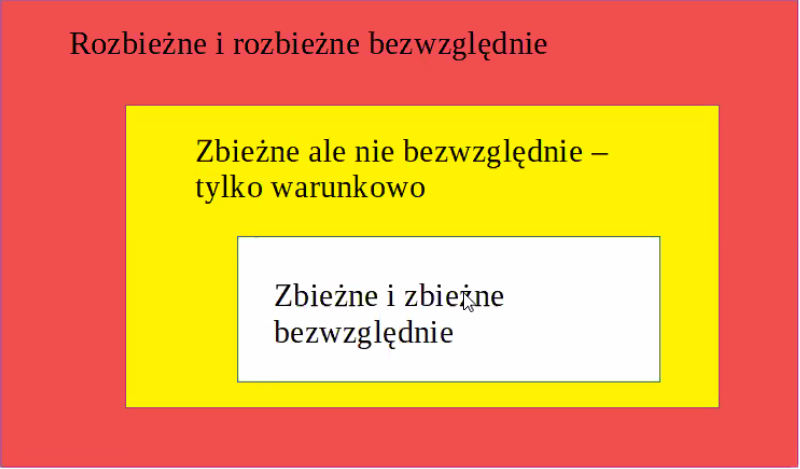
\includegraphics[scale=0.6]{rozbiezneirozbiezne.png}
\end{center}

\textbf{Przykład} 

Całka $ \int\limits_{1}^{\infty} \frac{\sin x}{\sqrt[3]{x^4}} \,dx $ jest zbieżna bezwzględnie, bo biorąc
$ \int\limits_{1}^{\infty} \left| \frac{\sin x}{\sqrt[3]{x^4}} \right| \,dx $ i używając kryterium porównawczego mamy

$$ 0 \leq \left| \frac{\sin x}{\sqrt[3]{x^4}} \right| = \frac{|\sin x|}{x^{\frac{4}{3}}} \leq \frac{1}{x^{\frac{4}{3}}} $$

a całka $ \int\limits_{1}^{\infty} \frac{1}{x^{\frac{4}{3}}} \,dx $ jest zbieżna bo $ \frac{4}{3} > 1 $.
Zatem $ \int\limits_{1}^{\infty} \left| \frac{\sin x}{\sqrt[3]{x^4}} \right| \,dx $ jest zbieżna, a stąd
$ \int\limits_{1}^{\infty} \frac{\sin x}{\sqrt[3]{x^4}} \,dx $ też jest zbieżna.

\section{Szeregi liczbowe}

Dany jest ciąg liczbowy $ a_1, a_2, ..., a_n, ... $

Tworzymy jego ciąg sum częściowych :

$$ S_1 = a_1, \ \ S_2 = a_1 + a_2, \ \ S_n = a_1 + a_2 + ... + a_n = \sum\limits_{k = 1}^{n} a_k $$

Jeżeli istnieje granica $ S = \lim_{n \to \infty} S_n $ (skończona lub nieskończona) to oznaczamy ją symbolem 
$ \sum_{k = 1}^{\infty} a_k $. \\

W ogólnym przypadku możemy wziąć ciąg, który zaczyna się od dowolnej liczby całkowitej \linebreak $ n_0 $ : $ a_{n_0}, a_{n_0 + 1}, ..., a_n, ... $
i jego sum częściowych

$$ S_n = a_{n_0}, \ \ S_{n_0 + 1} = a_{n_0} + a_{n_0 + 1}, \ \ S_n = a_{n_0} + a_{n_0 + 1} + ... + a_n = \sum\limits_{k = n_0}^{n} a_k, \ n \geq n_0 $$

$ S = \lim_{n \to \infty} S_n $ jest oznaczana przez $ \sum\limits_{k = n_0}^{\infty} a_k $. \\

Definicja. Dla ustalonego $ n_0 \in \mathbb{Z} $ obiekt $ \sum\limits_{k = n_0}^{\infty} a_k $ nazywamy \underline{szeregiem liczbowym},
a wartość S (gdy istnieje) jego \underline{sumą}, oznaczaną także przez $ \sum\limits_{k = n_0}^{\infty} a_k $. Mamy wtedy

$$ S_n = a_{n_0}, \ \ S_{n_0 + 1} = a_{n_0} + a_{n_0 + 1}. \ \ S_n = a_{n_0} + a_{n_0 + 1} + ... + a_n + ... = 
\sum\limits_{k = n_0}^{\infty} a_k = \lim_{n \to \infty} \sum\limits_{k = n_0}^{n} a_k = \lim_{n \to \infty} S_n $$

gdzie

\begin{itemize}
    \item $ S_n $ to $n$ - ta suma szeregu,
    \item $ a_n $ to $n$ - ty wyraz szeregu. \\
\end{itemize}

Terminologia dotycząca sumy $S$ jest taka, jak dla ciągów. Są 3 przypadki : 

\begin{enumerate}
    \item $S$ jest liczbą. Wtedy dany szereg jest \underline{zbieżny} (do $S$).
    \item $S = \infty$ lub $S = -\infty$. Wtedy dany szereg jest \underline{rozbieżny} (do $\infty$ lub $-\infty$).
    \item $ S = \lim_{n \to \infty} S_n $ nie istnieje. Wtedy dany szereg jest \underline{rozbieżny}. \\
\end{enumerate}

Przykłady

$$ \frac{1}{2^1} + \frac{1}{2^2} + \frac{1}{2^3} + ... + \frac{1}{2^n} + ... = \suminfty{1} \frac{1}{2^n} 
\textrm { - szereg zbieżny do 1}$$

$$ \frac{1}{2} + \frac{1}{3} + ... + \frac{1}{n} + ... = \sum\limits_{n = 2}^{\infty} \frac{1}{n} 
\textrm { - szereg rozbieżny do } \infty$$

$$ 1 - 1 + 1 - 1 + 1 - 1 + ... = \sum\limits_{n = 0}^{\infty} (-1)^n \textrm{ - szereg rozbieżny} $$

Uwaga. Każdy szereg zaczynający się od indeksu $ n_0 \in \mathbb{Z} $ można przekształcić tak, by zaczynał się od indeksu 1.
Wynika to z równości

$$ \sum\limits_{n = n_0}^{\infty} a_n = \suminfty{1} a_{n + n_0 - 1} $$

$$ \frac{1}{2} + \frac{1}{3} + ... + \frac{1}{n} + ... = \sum\limits_{n = 2}^{\infty} \frac{1}{n} = \sum\limits_{n = 2}^{\infty} a_n
= \suminfty{1} a_{n + 1} = \suminfty{1} \frac{1}{n + 1} $$

\subsection*{Obliczanie sum szeregów}
\addcontentsline{toc}{subsection}{Obliczanie sum szeregów}

Jest to zadanie trudne, a najczęściej niemożliwe, gdyż trudno jest znaleźć bezpośredni wzór na sumy częściowe $S_n$. \\

Niektóre przypadki szczególne.

\begin{enumerate}
    \item Ciąg geometryczny i szereg geometryczny.
    \begin{itemize}
        \item 
        $ a_n = a_1 \cdot q^{n-1} $, gdzie $q$ jest ilorazem ciągu (czyli $a_{n+1} = a_n \cdot q , \ n \geq 1$).
        
        Wtedy

        $$ S_n = a_1 + a_2 + ... + a_n = a_1 \cdot \frac{1 - q^n}{1 - q}, q \neq 1 \ oraz \ S_n = na_1, \ q = 1 $$

        To oznacza, że dla $ a_1 \neq 0 $,

        \item szereg jest zbieżny dla $ -1 < q < 1 $ i jego suma jest $ S = \frac{a_1}{1 - q} $,
        \item szereg jest rozbieżny do $\infty$ lub $-\infty$ dla $ q \geq 1 $, znak zależy od znaku $a_1$,
        \item szereg jest rozbieżny (suma nie istnieje) dla $ q \leq -1 $ \\
    \end{itemize}

    Stąd np.

    $$ \frac{1}{2^1} + \frac{1}{2^2} + \frac{1}{2^3} + ... + \frac{1}{2^n} + ... = \suminfty{1} \frac{1}{2^n} =
    \frac{ \frac{1}{2} }{ 1 - \frac{1}{2} } = 1 \ \textrm{, bo tutaj} \ a_1 = q = \frac{1}{2} $$

    \item Szeregi o wyrazie ogólnym postaci \\
    $ a_n = f(n + 1) - f(n)$ lub $ a_n = f(n) - f(n + 1) $, gdzie $f$ jest pewną funkcją.

    W bardziej ogólnej postaci \\
    \quad $ a_n = f(n + k) - f(n) $ lub $ a_n = f(n) - f(n + k) $, gdzie $ k \in \mathbb{N}^+ $ to tzw. krok. \\
    
    Takie szeregi to tzw. szeregi \underline{teleskopowe} (telescoping series).

    Przykłady

    $$ \suminfty{1} \left( \frac{1}{n} - \frac{1}{n + 1} \right) \ \textrm{- tutaj} \ f(x) = \frac{1}{x} $$

    $$ \suminfty{1} \left( \sqrt{n + 1} - \sqrt{n} \right) \ \textrm{- tutaj} \ f(x) = \sqrt{x} $$

    $$ \suminfty{1} \left( \arctan(n) - \arctan(n+2) \right) \ \textrm{- tutaj} \ f(x) = \arctan x $$

    Dla takich szeregów łatwo wyznacza się wzór na $S_n$. Wyrazy wewnętrzne się upraszczają i zostaje: \\
    suma $k$ pierwszych wartości, \ $f$ suma $k$ ostatnich wartości $f$ (lub na odwrót) \\

\end{enumerate}

Na przykład dla $ \suminfty{1} \left( f(n) - f(n + 1)) \right) $ mamy

$$ S_n = f(1) - \textcolor{red}{f(2)} + \textcolor{red}{f(2)} - \textcolor{blue}{f(3)} + \textcolor{blue}{f(3)} - 
\textcolor{green}{f(4)} + ... + \textcolor{purple}{f(n)} - f(n + 1) = f(1) - f(n + 1) $$.

Jeżeli istnieje granica $ G = \lim_{x \to \infty} f(x) $ to mamy

$$ S = \lim_{n \to \infty} S_n = \lim_{n \to \infty} \left( f(1) - f(n + 1) \right) = f(1) - G $$ \\

Przykład. Wyznaczyć sumę $ \suminfty{1} \frac{1}{n^2 + n} $

Wyraz ogólny nie ma postaci różnicy więc trzeba ją stworzyć.

Używając rozkładu na ułamki proste dostajemy

$$ \frac{1}{n^2 + n} = \frac{1}{n(n+1)} = \frac{A}{n} + \frac{B}{n+1} = ... = \frac{1}{n} - \frac{1}{n+1} $$

Zatem 

$$ \suminfty{1} \frac{1}{n^2 + n} = \sum\limits_{n=1}^{\infty} \left( \frac{1}{n} - \frac{1}{n+1} \right) $$

I to daje

$$ S_n = \left( \frac{1}{1} - \frac{1}{2} \right) + \left( \frac{1}{2} - \frac{1}{3} \right) + \left( \frac{1}{3} - \frac{1}{4} \right)
+ ... + \left( \frac{1}{n} - \frac{1}{n+1} \right) = \frac{1}{1} - \frac{1}{n+1}  $$ 

$$ \lim_{n \to \infty} S_n = 1 = \suminfty{1} \frac{1}{n^2 + n} $$

\subsection*{Własności szeregów zbieżnych}
\addcontentsline{toc}{subsection}{Własności szeregów zbieżnych}

\textbf{Twierdzenie}

Jeżeli szeregi $ \sum\limits_{n = n_0}^{\infty} a_n $ oraz $ \sum\limits_{n = n_0}^{\infty} b_n $ są zbieżne to zbieżne są szeregi
$ \sum\limits_{n = n_0}^{\infty} (a_n + b_n) $ \linebreak oraz $ \sum\limits_{n = n_0}^{\infty} (c \cdot a_n), \ c \in \mathbb{R} $. \\

Ponadto

\begin{itemize}
    \item $ \sum\limits_{n = n_0}^{\infty} (a_n \pm b_n) = \sum\limits_{n = n_0}^{\infty} a_n \pm \sum\limits_{n = n_0}^{\infty} b_n $
    \item $ \sum\limits_{n = n_0}^{\infty} (c \cdot a_n) = c \sum\limits_{n = n_0}^{\infty} a_n $ \\
\end{itemize}

Prawdziwe są także analogiczne twierdzenia prowadzące do arytmetyki granic nieskończonych, gdy nie pojawiają się symbole nieoznaczone.
Na przykład gdy $ \sum\limits_{n = n_0}^{\infty} a_n = \infty $ oraz $ \sum\limits_{n = n_0}^{\infty} b_n = b \in \mathbb{R} $ to 

$$ \sum\limits_{n = n_0}^{\infty} (a_n \pm b_n) = \sum\limits_{n = n_0}^{\infty} a_n \pm \sum\limits_{n = n_0}^{\infty} b_n = \infty $$ \\

Natomiast gdy $ \sum\limits_{n = n_0}^{\infty} a_n = \sum\limits_{n = n_0}^{\infty} b_n = \infty $ to
$ \sum\limits_{n = n_0}^{\infty} (a_n - b_n) $ może być zarówno zbieżny jak i rozbieżny i nie ma sensu równość

$$ \sum\limits_{n = n_0}^{\infty} (a_n - b_n) = \sum\limits_{n = n_0}^{\infty} a_n - \sum\limits_{n = n_0}^{\infty} b_n $$ \\

\textbf{Twierdzenie}

Zmiana wartości $n_0$ nie wpływa na zbieżność/rozbieżność szeregu $ \sum\limits_{n = n_0}^{\infty} a_n $.

Może mieć wpływ na wartość jego sumy. \\

Stąd wynika np., że szeregi $ \suminfty{1} a_n $ i $ \sum\limits_{n = 100}^{\infty} a_n $ są albo oba zbieżne
albo oba rozbieżne do $ \infty $ lub $-\infty$ albo oba rozbieżne.

To też oznacza, że na podstawie kilku pierwszych wyrazów ciągu/szeregu

\textbf{NIC NIE MOŻNA POWIEDZIEĆ} o jego zbieżności \\

\textbf{Popularny błąd}

"Liczymy wartości $ a_1, a_2, a_3, a_4, a_5$ . Wychodzi ciąg malejący i dodatni.

\textcolor{red}{Zatem szereg jest zbieżny}". \textbf{GAME OVER...} \\

\textbf{Twierdzenie}

Dla ustalonego $ n_0 \in \mathbb{N}^+ $ i $ p \in \mathbb{R} $ szereg $ \sum\limits_{n = n_0}^{\infty} \frac{1}{n^p} $
jest zbieżny dla $ p > 1 $ i rozbieżny do $\infty$ dla $p \leq 1$.  \\

W przypadku kiedy sumy szeregu nie da się wyznaczyć w sposób dokładny można to zrobić w sposób przybliżony, pod warunkiem, że wiemy,
że szereg jest zbiezny. \\

Kryteria zbieżności to twierdzenia opisujące warunki dostateczne zbieżności lub rozbieżności danej klasy szeregów. Najczęściej mają postać
implikacji ale \textbf{NIE} równoważności. \\

Oznacza to zwykle własności postaci

\quad warunek zachodzi $ \Rightarrow $ szereg jest zbieżny/rozbieżny,

\quad warunek nie zachodzi $\Rightarrow$ nic nie wiemy o zbieżności/rozbieżności szeregu \\

\subsection*{Popularne kryteria zbieżności szeregów}
\addcontentsline{toc}{subsection}{Popularne kryteria zbieżności szeregów}

0. Warunek konieczny zbieżności szeregów \\ 

\textbf{Twierdzenie}

Jeżeli szereg $ \sum\limits_{n = n_0}^{\infty} a_n $ jest zbieżny to $ \lim_{n \to \infty} a_n = 0 $. \\

Dowód 

Dla $ n \geq n_0 + 1 $ mamy $ S_n = a_{n_0} + a_{n_0 + 1} + ... + a_{n - 1} + a_n $ oraz 
$ S_{n - 1} = a_{n_0} + a_{n_0 + 1} + ... + a_{n - 1} $,

Stąd

$$ S_n - S_{n - 1} = a_n $$ \\

Jeżeli szereg $ \sum\limits_{n = n_0}^{\infty} a_n $ jest zbieżny to $ \lim_{n \to \infty} S_n = \lim_{n \to \infty} S_{n - 1} = S \in \mathbb{R} $.
To daje

$$ \lim_{n \to \infty} a_n = \lim_{n \to \infty} (S_n - S_{n - 1}) = \lim_{n \to \infty} S_n - \lim_{n \to \infty} S_{n - 1} = S - S = 0 $$ \\

Transpozycja tego twierdzenia daje warunek równoważny do zastosowania praktycznego :

Jeżeli $ \lim_{n \to \infty} a_n \neq 0 $ to szereg $ \sum\limits_{n = n_0}^{\infty} a_n $ nie jest zbiezny przy czym

\begin{itemize}
    \item gdy $ \lim_{n \to \infty} a_n > 0 $ to $ \sum\limits_{n = n_0}^{\infty} a_n = \infty $
    \item gdy $ \lim_{n \to \infty} a_n < 0 $ to $ \sum\limits_{n = n_0}^{\infty} a_n = -\infty $ 
\end{itemize}

\textbf{Uwaga. To jest tylko implikacja!}

Jeżeli $ \lim_{n \to \infty} a_n = 0 $ to jeszcze \textbf{NIC NIE WIEMY} o szeregu.

Na przykład szeregi $ \sum\limits_{n = n_0}^{\infty} \frac{1}{n^p} $ mają $ \lim_{n \to \infty} \frac{1}{n^p} = 0 $
dla wszystkich $ p > 0 $ ale niektóre z tych szeregów są zbieżne, a niektóre rozbieżne. \\

\textbf{Popularny błąd}

"$\lim_{n \to \infty} a_n = 0 $ \textcolor{red}{zatem szereg jest zbieżny}". \textbf{GAME OVER...} \\

Szeregi o wyrazach nieujemnych

$$ \sum\limits_{n = n_0}^{\infty} a_n, \ a_n \geq 0 $$

Wtedy $ S_n = a_{n_0} + a_{n_0 + 1} + ... + a_{n - 1} + a_n $ jest ciągiem niemalejącym zatem suma szeregu
$ \sum\limits_{n = n_0}^{\infty} a_n = \lim_{n \to \infty} S_n $ zawsze istnieje. Może być to liczba lub $\infty$.

Podobnie dla szeregów o wyrazach niedodatnich $ \sum\limits_{n = n_0}^{\infty} a_n, \ a_n \leq 0 $, suma zawsze istnieje
i rozbieżność oznacza rozbieżność do $-\infty$. \\

Przykład. Następujące szeregi nie są zbieżne

$$ \suminfty{1} 1, \ \ \suminfty{1} (n^2 + 2n), \ \
\suminfty{1} \frac{n+1}{n+2}, \ \ \suminfty{1} \left(1 + \frac{1}{n} \right)^n , \ \ 
\suminfty{1} (-1)^n , \ \ \suminfty{1} \sin n$$

Dla szeregów o wyrazach nieujemnych mamy dwa kolejne kryteria zbieżności.

\begin{enumerate}
    \item Kryterium porównawcze
    \item Kryterium ilorazowe \\
\end{enumerate} 

\subsection*{Twierdzenie (kryterium porównawcze)}
\addcontentsline{toc}{subsection}{Twierdzenie (kryterium porównawcze)}

Dane są dwa szeregi $ \sum\limits_{n = n_0}^{\infty} a_n $ oraz $ \sum\limits_{n = n_0}^{\infty} b_n $. Wtedy zachodzą nastepujące
własności.

\begin{enumerate}
    \item (Przypadek zbieżności) Gdy $ \forall n \geq k \geq n_0 \quad 0 \leq a_n \leq b_n $ i $ \sum\limits_{n = n_0}^{\infty} b_n $
    jest zbieżny to $ \sum\limits_{n = n_0}^{\infty} a_n $ też jest zbieżny. Ponadto
    $ 0 \leq \sum\limits_{n = n_0}^{\infty} a_n \leq \sum\limits_{n = n_0}^{\infty} b_n $
    
    \item (Przypadek rozbieżności) Gdy $ \forall n \geq k \geq n_0 \quad 0 \leq b_n \leq a_n $ i $ \sum\limits_{n = n_0}^{\infty} b_n $
    jest rozbieżny to $ \sum\limits_{n = n_0}^{\infty} a_n $ też jest rozbieżny. Ponadto
    $ \sum\limits_{n = n_0}^{\infty} a_n = \sum\limits_{n = n_0}^{\infty} b_n = \infty $

    \item (Przypadek wątpliwy). Gdy $ \forall n \geq k \geq n_0 \quad 0 \leq a_n \leq b_n $ ale $ \sum\limits_{n = n_0}^{\infty} b_n $ jest
    rozbieżny to \textbf{NIC NIE WIEMY} o zbieżności $ \sum\limits_{n = n_0}^{\infty} a_n $

    \item (Przypadek wątpliwy). Gdy $ \forall n \geq k \geq n_0 \quad 0 \leq b_n \leq a_n $ ale $ \sum\limits_{n = n_0}^{\infty} b_n $ jest
    zbieżny to \textbf{NIC NIE WIEMY} o zbieżności $ \sum\limits_{n = n_0}^{\infty} a_n $ \\
\end{enumerate}

Uwagi

\begin{itemize}
    \item $ \sum\limits_{n = n_0}^{\infty} a_n $ jest szeregiem z zadania, $ \sum\limits_{n = n_0}^{\infty} b_n $ tworzymy sami
    \item Porównujemy najczęściej z szeregiem geometrycznym $ \sum\limits_{n = n_0}^{\infty} q^n $ lub z szeregami
    $ \sum\limits_{n = n_0}^{\infty} \frac{1}{n^p} $. Wtedy $a_n$ często ma postać ułamków i możemy spróbować wziąć $b_n$ jako

    \quad \textbf{C $\cdot$ iloraz najwyższych potęg z licznika i mianownika $a_n$} 

    \item Trzeba uważać aby nierówność między $a_n$ i $b_n$ była prawdziwa i nie zapomnieć o dolnym ograniczeniu (0). Ma być
    tak jak w \underline{twierdzeniu o trzech ciągach}

    \item Kryterium nie zawsze jest wygodne w użyciu i trzeba uważać, by nie dostać przypadku wątpliwego, bo wtedy \textbf{trzeba zaczynać od nowa}
    
    \item Warto sprawdzić opisany wyżej iloraz najwyższych potęg i na tej podstawie przewidzieć czy chcemy udowodnić zbieżność
    czy rozbieżność. To pomaga skonstruować odpowiednią nierówność między $a_n$ i $b_n$.
\end{itemize}

\textbf{Popularny błąd : } odpowiedź na podstawie przypadku wątpliwego

Na przykład dla szeregu $ \suminfty{1} \frac{1}{n + \sqrt{n}} : $

"Mamy $ 0 \leq \frac{1}{n + \sqrt{n}} \leq \frac{1}{n} $ i szereg $ \suminfty{1} \frac{1}{n} $
jest rozbieżny \textcolor{red}{zatem szereg $\suminfty{1} \frac{1}{n + \sqrt{n}}$ jest rozbieżny}". \\

\textbf{GAME OVER...} To jest przypadek nr 3 (wątpliwy) \\

Przykład

$$ \sum\limits_{n = 4}^{\infty} \frac{2n - 3}{n^3 - 1} $$

Przewidywanie zbieżności/rozbieżności:

Iloraz najwyższych potęg licznika i mianownika to $ \frac{n}{n^3} = \frac{1}{n^2} $, a szereg $ \sum\limits_{n = 4}^{\infty} \frac{1}{n^2} $
jest zbieżny, bo $ 2 > 1 $. Zatem chcemy udowodnić zbieżność (przypadek 1).

Potrzebujemy więc $ \sum\limits_{n = 4}^{\infty} b_n $ i nierówności $ 0 \leq \frac{2n - 3}{n^3 - 1} \leq b_n $.

Chcemy zwiększyć wyrażenie $ \frac{2n - 3}{n^3 - 1} $ ale tak, by \textbf{zostały najwyższe potęgi}.

Można zwiększyć \underline{licznik} oraz \underline{zmniejszyć mianownik}.

Zwiększamy licznik poprzez wyrzucenie 3.

Zmniejszamy mianownik poprzez zastąpienie 1 czymś większym : wyrażeniem z najwyższą potęgą. Nie można jednak wziąć całego $n^3$
, bo będzie 0 w mianowniku.

Wygrywa wzięcie $ C \cdot n^3 $ np. $ \frac{1}{2} n^3 $, bo dla $ n \geq 4 $ mamy $ \frac{1}{2} n^3 \geq 1 $.

To wszystko daje dla $ n \geq 4 $

$$ 0 \leq \frac{2n - 3}{n^3 - 1} \leq \frac{2n}{n^3 - \frac{1}{2} n^3} $$

Czyli

$$ b_n = \frac{2n}{n^3 - \frac{1}{2}n^3} = 4 \cdot \frac{1}{n^2} $$

\textbf{DZIURA W SKRYPCIE}

\subsection*{Twierdzenie (kryterium ilorazowe)}
\addcontentsline{toc}{subsection}{Twierdzenie (kryterium ilorazowe)}

Dane są dwa szeregi $ \sum\limits_{n = n_0}^{\infty} a_n $ oraz $ \sum\limits_{n = n_0}^{\infty} b_n $.
Ponadto $ \forall n \geq n_0 \ a_n, b_n > 0 $.

Jeżeli istnieje granica $ \lim_{n \to \infty} \frac{a_n}{b_n} $ i jest \textbf{liczbą dodatnią} to wtedy oba
szeregi są zbieżne albo oba rozbieżne do $\infty$. \\

Uwagi

\begin{itemize}
    \item Ciąg $b_n$ tworzymy podobnie jak dla kryterium porównawczego.
    \item Nie ma problemu z nierównościami :) ale za to trzeba umiećl liczyć granice.
    \item Granica nie może być ani 0 ani $\infty$: \ $ \lim_{n \to \infty} \frac{a_n}{b_n} = L \in (0, \infty) $.
    
    \textbf{Nie wystarczy warunek $L > 0$ bo $\infty$ także jest $ > 0$.}
    \item Rozwiązanie textbf{musi zawierać wniosek} "granica ilorazu jest liczbą dodatnią więc oba
    \textbf{szeregi} są zbieżne lub oba rozbieżne" - bez tego będzie niepełne
    
    \item Kryterium zwykle jest wygodniejsze niż porównawcze ale są przykłady, które pójdą z porównawczego ale nie z
    ilorazowego, bo granica ilorazu nie istnieje
    
    Np. \ $ \suminfty{1} \frac{2 + \sin n}{n} $.
\end{itemize}

Przykłady

Poprzedni przykład raz jeszcze 

$$ \sum\limits_{n = 4}^{\infty} \frac{2n - 3}{n^3 - 1} $$

Bierzemy $ b_n = \frac{n}{n^3} = \frac{1}{n^2} $

$$ \dfrac{a_n}{b_n} = \dfrac{\dfrac{2n - 3}{n^3 - 1}}{\dfrac{1}{n^2}} = \dfrac{2n^3 - 3n^2}{n^3 - 1}
= \dfrac{2 - \dfrac{3}{n}}{1 - \dfrac{1}{n^3}} $$ \\

Stąd $ \lim_{n \to \infty} \frac{a_n}{b_n} = 2 $ - liczba dodatnia.

Zatem oba szeregi są zbieżne lub oba są rozbieżne.

Dalej już analiza $ \sum\limits_{n = 4}^{\infty} \frac{1}{n^2} $ i wniosek jak w kryterium porównawczym :

$ \sum\limits_{n = 4}^{\infty} b_n = \sum\limits_{n = 4}^{\infty} \frac{1}{n^2} $ jest zbieżny bo $ 2 > 1 $.
Zatem $ \sum\limits_{n = 4}^{\infty} \frac{2n - 3}{n^3 - 1} $ też jest zbieżny. \\\\

Przykłady o postaci funkcji złożonej $ \sum\limits_{n = n_0}^{\infty} f(b_n) $,

gdzie $ \lim_{n \to \infty} b_n = 0^+ $ oraz $ \lim_{x \to 0^+} f(x) = 0^+ $.

Nowym szeregiem jest szereg z funkcji wewnętrznej $ \sum\limits_{n = n_0}^{\infty} b_n $.

Liczymy granicę 

$$ \lim_{n \to \infty} \frac{f(b_n)}{b_n} = \lim_{x=b \to 0^+} \frac{f(x)}{x} \left[ \frac{0}{0} \right] $$

przy użyciu granic podstawowych lub reguły de l'Hospitala. \\

Na przykład

$$ \suminfty{1} \left( \sqrt[n]{2} - 1 \right) $$

Mamy $$ \suminfty{1} \left( \sqrt[n]{2} - 1 \right) = \suminfty{1} \left( 2^{\frac{1}{n}} - 1 \right) $$

Więc bierzemy $ b_n = \frac{1}{n} > 0 $.

Liczymy granicę

$$ \lim_{n \to \infty} \frac{2^{\frac{1}{n}} - 1}{\frac{1}{n}} = \lim_{x = \frac{1}{n} \to 0^+} \frac{2^x - 1}{x} = \ln 2 $$ \\

Jest to liczba dodatnia więc oba szeregi są zbieżne lub oba są rozbieżne.

$ \suminfty{1} \frac{1}{n} = \infty $ więc $ \suminfty{1} \left( \sqrt[n]{2} - 1 \right) = \infty $. \\ \\

3. Kryterium Cauchy'ego.

4. Kryterium d'Alemberta \\

Działają dla szeregów o dowolnych wyrazach. Teza obu kryteriów jest taka sama ale liczymy granice innych wyrażeń.


\subsection*{Twierdzenie (kryterium Cauchy'ego)}
\addcontentsline{toc}{subsection}{Twierdzenie (kryterium Cauchy'ego)}

Dany jest szereg $ \sum\limits_{n = n_0}^{\infty} a_n $ taki, że istnieje granica $ q = \lim_{n \to \infty} \sqrt[n]{|a_n|} $. Wtedy

\begin{enumerate}
    \item Gdy $ 0 \leq q < 1 $ to szereg jest zbieżny.
    \item Gdy $ q > 1 $ to szereg jest rozbieżny
    \item \textbf{(Przypadek wątpliwy)}. Gdy q = 1 to \textbf{NIC NIE WIEMY} o zbieżności szeregu. \\
\end{enumerate}

\textbf{Uwagi}

\begin{itemize}
    \item Do wyznaczenia $q$ przydają się następujące właśności granic
    
    a) Gdy $ \lim_{n \to \infty} a_n $ jest \textbf{liczbą dodatnią} to $ \lim_{n \to \infty} \sqrt[n]{a_n} = 1 $.

    b) $ \forall p \in \mathbb{R} \ \lim_{n \to \infty} \sqrt[n]{n^p} = 1 $.

    \item \textbf{$q$ nie może być ujemne}. $q$ ujemne zwykle oznacza brak modułu na $a_n$.
\end{itemize}


\subsection*{Twierdzenie (kryterium d'Alemberta)}
\addcontentsline{toc}{subsection}{Twierdzenie (kryterium d'Alemberta)}

Dany jest szereg $ \sum\limits_{n = n_0}^{\infty} a_n, \ a_n \neq 0 $, taki, że istnieje granica
$ q = \lim_{n \to \infty} \left| \frac{a_{n + 1}}{a_n} \right| $. Wtedy

\begin{enumerate}
    \item Gdy $ 0 \leq q < 1 $ to szereg jest zbieżny.
    \item Gdy $ q > 1 $ to szereg jest rozbieżny
    \item \textbf{(Przypadek wątpliwy)}. Gdy q = 1 to \textbf{NIC NIE WIEMY} o zbieżności szeregu. \\
\end{enumerate}

\begin{itemize}
    \item \textbf{$q$ nie może być ujemne}. $q$ ujemne zwykle oznacza brak modułu na $a_n$.
    
    \item W obu kryteriach szerergi $ \sum\limits_{n = n_0}^{\infty} \frac{1}{n^p} $ pokazują, że $ q = 1$ nic nie daje. \\
\end{itemize}

Przykłady

$$ \suminfty{1} \frac{20^n}{n!} $$

Tutaj $ a_n = \frac{20^n}{n!} > 0 $ oraz $ a_{n + 1} = \frac{20^{n + 1}}{(n + 1)!} $. Zatem z kryterium d'Alemberta

$$ q = \lim_{n \to \infty} \left| \frac{a_{n + 1}}{a_n} \right| = \frac{ \dfrac{20^{n + 1}}{(n+1)!} }{ \dfrac{20^n}{n!} } $$ \\

$$ \suminfty{1} \left( 2\arcsin \frac{1 - n}{2n + 1} \right)^n $$

Tutaj chcemy użyć kryterium Cauchy'ego.

$$ \sqrt[n]{|a_n|} = \sqrt[n]{ \left| \left( 2\arcsin \frac{1-n}{2n+1} \right)^n \right| } 
= \sqrt[n]{ \left| 2\arcsin \frac{1-n}{2n+1} \right|^n } = \left| 2\arcsin \frac{1-n}{2n+1} \right|
= \left| 2\arcsin \frac{ \dfrac{1}{n} - 1  }{ 2 + \dfrac{1}{n} } \right| $$

Stąd 

$$ q = \lim_{n \to \infty} \sqrt[n]{|a_n|} = \left| 2\arcsin \left( -\frac{1}{2} \right) \right|
= \left| 2 \left( - \frac{\pi}{6} \right) \right| = \frac{\pi}{3} $$

$q > 1$ więc szereg jest rozbieżny.


\subsection*{Twierdzenie (kryterium całkowe)}
\addcontentsline{toc}{subsection}{Twierdzenie (kryterium całkowe)}

Dany jest szereg $ \sum\limits_{n = n_0}^{\infty} a_n $. Jeżeli na $ [x_0, \infty), \ x_0 \geq n_0 $ istnieje funkcja $f$
taka, że 

\begin{itemize}
    \item $ f(n) = a_n, \ n \geq x_0 $,\
    \item $f$ jest nieujemna na $[x_0, \infty)$,
    \item $f$ jest nierosnąca na $[x_0, \infty)$,
\end{itemize}

to całka niewłaściwa $ \int\limits_{x_0}^{\infty} f(x) \,dx $ i szereg $ \sum\limits_{n = n_0}^{\infty} a_n $ są
jednocześnie skończone lub jednocześnie rozbieżne do $\infty$. \\

Uwagi do kryterium

\begin{itemize}
    \item Najczęściej $ x_0 = n_0 $.
    \item Kryterium jest ważne z punktu widzenia teorii, gdyż wiele innych własności szeregów z niego wynika.
    Na przykład, gdy $x_0 = n_0$ to
    $$ \int\limits_{n_0}^{\infty} f(x) \,dx \leq \sum\limits_{n = n_0}^{\infty} a_n \leq 
    a_{n_0} + \int\limits_{n_0}^{\infty} f(x) \,dx $$
    To pozwala oszacować sumę szeregu.

    \item Sens użycia kryterium: nie umiemy policzyć sumy szeregu ale umiemy \textbf{obliczyć} całkę
    $ \int\limits_{x_0}^{\infty} f(x) \,dx = \lim_{T \to \infty} \int\limits_{x_0}^{T} f(x) \,dx $. Stosujemy to
    kryterium tylko wtedy, gdy zamierzamy liczyć tę całkę.

    \item Z praktycznego punktu widzenia kryterium jest najczęściej \textbf{najmniej wygodnie} do zastosowania.
    Opłaca się je stosować głównie wtedy, gdy szereg zawiera wyrażenie $\ln n$. \\
\end{itemize}

Przykład

Dla ustalonego $ n_0 \in \mathbb{N}^+ $ i $p > 0$ dowodzimy znany już wynik dla szeregu $ \sum\limits_{n = n_0}^{\infty} \frac{1}{n^p} $
zbieżny dla $p > 1$ oraz rozbieżny do $\infty$ dla $p \leq 1$. \\

Tutaj bierzemy po prostu $ f(x) = \frac{1}{x^p}, \ x \in [n_0, \infty) $.

Dla $p > 0$ $f$ jest malejąca i nieujemna oraz $ f(n) = \frac{1}{n^p} $ 

Spełnione są wiec warunki użycia kryterium. Liczymy całkę $ \int\limits_{n_0}^{\infty} \frac{1}{x^p} \,dx $.

Było to już robione wcześniej i wiemy, że dla $p > 1$ jest liczbą, a dla $p \leq 1$ jest równa $\infty$.
Stąd szereg jest zbieżny dla $p > 1$ oraz rozbieżny do $\infty$ dla $0 < p \leq 1$. Dla $p \leq 0$ szereg jest rozbieżny,
bo nie spełnia warunku koniecznego zbieżności. \\

Uwaga do szeregów z wyrażeniem $\ln n$.

Dla dowolnego $p>0$ funkcja $\frac{\ln x}{x^p}, \ x \geq 2$, ma zbiór wartości $\left( 0, \frac{1}{p \cdot e} \right]$. Zatem

$$ \frac{\ln x}{x^p} \leq \frac{1}{p \cdot e} \Leftrightarrow \ln x \leq \frac{1}{p \cdot e} x^p $$

a stąd

$$ \ln n \leq \frac{1}{p \cdot e} n^p $$

Z oszacowaniem dolnym jest gorzej, bo nie ma pojedynczej funkcji elementarnej mniejszej od $\ln x$ i pozostaje oszacowanie
przez stałą np.

$$ \ln n \geq \frac{1}{2}, \quad n \geq 2  $$

To daje oszacowanie dla dowolnego $p>0$:

$$ \frac{1}{2} \leq \ln n \leq C \cdot n^p, \quad n \geq 2 $$

Tutaj $ C = \frac{1}{p \cdot e} $, a dla $ p \geq \frac{1}{e} $ wystarczy wziąć $C = 1$.

Często to oszacowanie pozwala uniknąć kryterium całkowego i zastąpienie go porównawczym, potrzeba tylko wziąć
odpowiednio małe p. \\

Przykład

Dla szeregu $ \sum\limits_{n = 2}^{\infty} \frac{\ln n}{n \sqrt[5]{n}} $ z kryterium porównawczego mamy

$$ 0 < \frac{\ln n}{n \sqrt[5]{n}} \leq \frac{Cn^p}{n \sqrt[5]{n}} = \frac{Cn^p}{n \cdot n^{0,2}} = \frac{C}{n^{1,2 - p}} $$

Wystarczy teraz wziąć $p < 0,2$ czyli np. $p = 0,1$ i zbadać szereg

$$ \sum\limits_{n=2}^{\infty} \frac{C}{n^{1,2 - 0,1}} = C \sum\limits_{n=2}^{\infty} \frac{C}{n^{1,1}} 
\ \ \textrm{--- zbieżny, bo} \ 1,1 > 1$$

Zatem wyjściowy szereg jest zbieżny


\subsection*{Zbieżność bezwzględna szeregów}
\addcontentsline{toc}{subsection}{Zbieżność bezwzględna szeregów}

Definicja. Szereg $ \sum\limits_{n=n_0}^{\infty} a_n$ jest \underline{zbieżny bezwzględnie}, gdy zbieżny jest szereg
$ \sum\limits_{n=n_0}^{\infty} |a_n|$. \\

Uwagi

\begin{itemize}
    \item Gdy wszystkie wyrazy $a_n$ są nieujemne to mamy $\sum\limits_{n=n_0}^{\infty} a_n = \sum\limits_{n=n_0}^{\infty} |a_n|$
    i definicja nie wnosi nic nowego. Sytuacja się zmienia gdy szereg ma zarówno wyrazy dodatnie jak i ujemne.
    \item Z nierówności $|S_n|= |a_{n_0} + a_{n_0+1} + ... + a_n| \leq |a_{n_0}| + |a_{n_0 + 1}| + ... + |a_n| $
    wynika nierówność $ \left| \sum\limits_{n=n_0}^{\infty} a_n \right| \leq \sum\limits_{n=n_0}^{\infty} |a_n| $
    ale równość nie musi zachodzić.

    Np. dla $ a_n = \left( -\frac{1}{2} \right)^n $ mamy $ \left| \sum\limits_{n=0}^{\infty} a_n \right| = \frac{2}{3} $
    \ ale \ $  \sum\limits_{n=0}^{\infty} |a_n| = 2 $

    Zatem $ \left| \sum\limits_{n=n_0}^{\infty} a_n \right| $ \ i \ $ \sum\limits_{n=n_0}^{\infty} |a_n| $ \textbf{to nie to samo}. \\
\end{itemize}

\textbf{Twierdzenie}

Jeżeli szereg jest bezwzględnie zbieżny to jest zbieżny (w zwykłym sensie).

Transpozycja tego twierdzenia daje warunek równoważny:

Jeżeli szereg $ \sum\limits_{n = n_0}^{\infty} a_n $ nie jest zbieżny to również nie jest zbieżny bezwzględnie, co oznacza
$ \sum\limits_{n=n_0}^{\infty} |a_n| = \infty $.

Twierdzenie odwrotne nie jest prawdziwe. Są szeregi zbieżne ale nie bezwzględnie, np.
$ \sum\limits_{n=1}^{\infty} \frac{(-1)^n}{n} $. Takie szeregi to tzw. szeregi \underline{zbieżne warunkowo}. \\

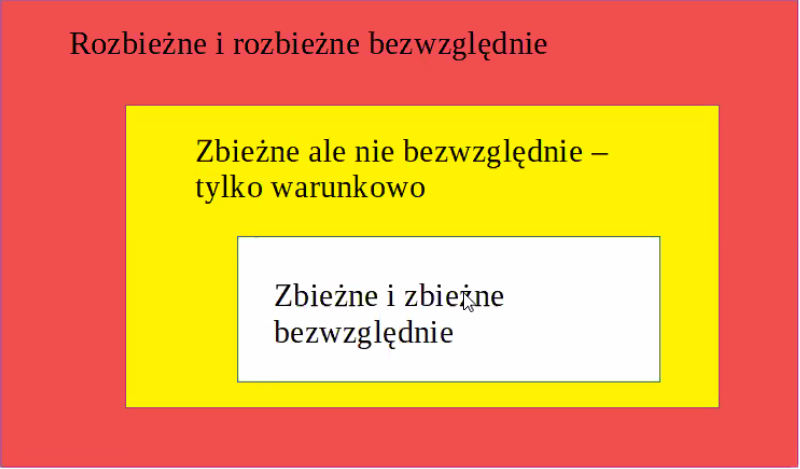
\includegraphics[scale=0.6]{rozbiezneirozbiezne.png} \\

Przykład 

Szereg $ \sum\limits_{n=1}^{\infty} \frac{\sin n}{\sqrt[3]{n^4}} $ jest zbieżny bezwzględnie, bo biorąc
$ \sum\limits_{n=1}^{\infty} \left| \frac{\sin n}{\sqrt[3]{n^4}} \right| $ i używając kryterium porównwawczego mamy

$$ 0 \leq \left| \frac{\sin n}{\sqrt[3]{n^4}} \right| = \frac{|\sin n|}{n^{\frac{4}{3}}} \leq \frac{1}{n^{\frac{4}{3}}} $$

a szereg $ \sum\limits_{n=1}^{\infty} \frac{1}{n^{\frac{4}{3}}} $ jest zbieżny, bo $ \frac{4}{3} > 1 $. 

Zatem
$ \sum\limits_{n=1}^{\infty} \left| \frac{\sin n}{\sqrt[3]{n^4}} \right| $, a stąd
$\sum\limits_{n=1}^{\infty} \frac{\sin n}{\sqrt[3]{n^4}}$ też jest zbieżny.


\subsection*{Szeregi naprzemienne}
\addcontentsline{toc}{subsection}{Szeregi naprzemienne}

Są to szeregi, w których na zmianę dodajemy i odejmujemy wyrazy dodatnie:

$ a_{n_0} - a_{n_0 + 1} + a_{n_0 + 2} - a_{n_0 + 3} + ... $ \ lub \ $ -a_{n_0} + a_{n_0 + 1} - a_{n_0 + 2} + a_{n_0 + 3} + ...  $ \
gdzie $a_n > 0$. \\

Postać ogólna :

$ \sum\limits_{n = n_0}^{\infty} (-1)^n \cdot a_n $ \ lub \ $ \sum\limits_{n = n_0}^{\infty} (-1)^{n+1} \cdot a_n $ \\

Przykłady

$$ \sqrt{2} - \sqrt{3} + \sqrt{4} - \sqrt{5} + ... = \sum\limits_{n=2}^{\infty} (-1)^n \sqrt{n} $$

$$ 1 - \frac{1}{2} + \frac{1}{3} - \frac{1}{4} + ... = \sum\limits_{n=1}^{\infty} \frac{(-1)^{n+1}}{n} $$ \\

Definicja

Szereg naprzemienny $ \sum\limits_{n = n_0}^{\infty} (-1)^n \cdot a_n $ \ lub \ $ \sum\limits_{n = n_0}^{\infty} (-1)^{n+1} \cdot a_n $
nazywany jest \underline{szeregiem Leibnitza}, jeżeli $a_n$ jest ciągiem nierosnącym i zbieżnym do 0.

Na przykład $ 1 - \frac{1}{2} + \frac{1}{3} - \frac{1}{4} + ... = \sum\limits_{n=1}^{\infty} \frac{(-1)^{n+1}}{n} $
jest szeregiem Leibnitza, bo tutaj $ a_n = \frac{1}{n} $ jest malejący i zbieżny do 0. \\

\textbf{Twierdzenie (Leibnitz)}

Każdy szereg Leibnitza jest zbieżny. \\

Uwagi

\begin{itemize}
    \item Twierdzenie to daje tylko zbieżność warunkową, nie gwarantuje bezwględnej
    \item Gdy ciąg $a_n$ nie dąży do 0 to szereg naprzemienny $ \sum\limits_{n = n_0}^{\infty} (-1)^n \cdot a_n $ jest
    rozbieżny, gdyż $(-1)^n a_n$ też nie dąży do 0. Wynika to z twierdzenia

    $$ \lim_{n \to \infty} a_n = 0 \Leftrightarrow \lim_{n \to \infty} (-1)^n a_n = 0 \Leftrightarrow \lim_{n \to \infty} |a_n| = 0$$

    \item Wystarczy, by ciąg $a_n$ był nierosnący dla $ \forall n \geq k \geq n_0$.
    \item Gdy ciąg $a_n$ zbiega do 0 ale nie jest nierosnący to \textbf{NIC NIE WIEMY} o zbieżności szeregu.
    \item Do badania czy $a_n$ jest nierosnący można próbować rozszerzyć $a_n$ do funkcji $f$ tak by $f(n) = a_n$.
    Potem --- pochodna itd.
    Gdy szereg naprzemienny jest zbieżny bezwzględnie to tw. Leibnitza nie jest potrzebne. \\
\end{itemize}

\textbf{Popularny błąd : } opisowanie "badanie" monotoniczności ciągu, bez obliczeń.

Na przykład dla ciągu $ a_n = \frac{n}{1000n + 1} $ :

"Ciąg $a_n$ jest \textcolor{red}{malejący}, bo mianownik \textcolor{red}{szybciej rośnie niż licznik}."

GAME OVER... \ Takie "rozwiązanie" jest jak \textbf{pisanie bajek} --- nie musi mieć \linebreak
\textbf{nic wspólnego z prawdą}.

Dla powyższego ciągu mianownik rzeczywiście szybciej rośnie niż licznik (i to 1000 razy!), a mimo to ciąg ten jest rosnący. \\

Przykład

$$ \sum\limits_{n=2}^{\infty} \frac{(-1)^n \cdot \ln n}{n} $$

Tutaj $ a_n = \frac{\ln n}{n} $. Rozszerzamy go do funkcji $ f(x) = \frac{\ln x}{x}, \ x \geq 2 $.

$$ f'(x) = \frac{1 - \ln x}{x^2} < 0 \Leftrightarrow x > e \approx 2,72 $$

Zatem $f$ jest malejąca dla $ x \in (e, \infty) $ czyli $a_n$ jest malejący dla $n \geq 3$.

Ponadto

$$ \lim_{x \to \infty} f(x) = \lim_{x \to \infty} \frac{\ln x}{x} = \left[ \frac{\infty}{\infty} \right][H]
= \lim_{x \to \infty} \frac{\frac{1}{x}}{1} = 0 $$

Zatem $ \lim_{n \to \infty} a_n = 0 $.

Mamy więc szereg naprzemienny, który z tw. Leibnitza jest zbieżny.

Nie jest jednak zbieżny bezwzględnie bo dla $ \sum\limits_{n=2}^{\infty} \left| \frac{(-1)^n \cdot \ln n}{n} \right|
= \sum\limits_{n=2}^{\infty} \frac{\ln n}{n} $ mamy z kryterium porównawczego $0 < \frac{0,5}{n} < \frac{\ln n}{n}$,
a szereg $ \sum\limits_{n=2}^{\infty} \frac{0,5}{n} $ jest rozbieżny.

Jest to więc szereg zbieżny warunkowo. \\

Podsumowanie : które kryterium zbieżności kiedy?

\begin{itemize}
    \item P --- porównawcze
    \item I --- ilorazowe
    \item C - Cauchy'ego
    \item A - d'Alemberta
    \item $\int$ --- całkowe
    \item ZB --- zbieżność bezwględna
    \item L - twierdzenie Leibnitza \\
\end{itemize}

\begin{table}[!htbp]
    \centering
    \begin{adjustbox}{width=0.9\textwidth}
    \begin{tabular}{|c|c|}
    \hline
    Wyrażenia występujące w $a_n$ & Sugerowane kryterium dla $ \sum\limits_{n=n_0}^{\infty} a_n $ \\[15pt] \hline
    Tylko potęgi $n$ lub pierwiastki z potęg $n$ & P \ \colorbox{yellow}{I} \ ale \colorbox{red}{NIGDY C A} \\[10pt] \hline 
    \underline{Te same} najwyższe potęgi $a_n$ w \underline{liczniku i mianowniku} & P \ \colorbox{yellow}{I} \ ale \colorbox{red}{NIGDY C A} \\[10pt] \hline
    \underline{Różne} najwyższe potęgi $a_n$ w \underline{liczniku i mianowniku} & P \ I \ \colorbox{yellow}{C \ A} \\[10pt] \hline
    funkcja złożona $ f(b_n), \ b_n \to 0 $ & \colorbox{yellow}{I} \ P \\[10pt] \hline
    n! & \colorbox{yellow}{A} \ P \\[10pt] \hline
    $n$ - ta sama potęga: $(...)^n$ & C \\[10pt] \hline
    Ciągi bez granicy, np. $\sin n$ & P \ (+ inne, gdy trzeba) \\[10pt] \hline
    $\ln n$ & \colorbox{yellow}{P} \ $\int$ \\[10pt] \hline
    $(-1)^n$ i ogólne $a_n$, o różnych znakach & ZB \ (+ inne, gdy trzeba) \ L \\[10pt] \hline
    \end{tabular}
\end{adjustbox}
\end{table}

\pagebreak

Przykłady do samodzielnego policzenia : \\

\begin{adjustbox}{width=0.7\textwidth}
    \begin{tabular}{ccc}
        $ \suminfty{1} \frac{\sqrt{n^2 + 3}}{n^3 + 2} $ & $ \suminfty{1} \frac{n^3 + 5}{n!} $ & $ \suminfty{1} \frac{2^n + 3^n}{n^2 \cdot 3^n + 1} $ \\
        \\
        $ \suminfty{1} \frac{2^n + 7 \cdot 3^n}{5^n - 4^n} $ & $ \suminfty{1} \left( \frac{2n+3}{3n+2} \right)^n $ & $ \suminfty{1} \arctan \frac{1}{\sqrt{n}} $ \\
        \\
        $ \suminfty{1} \frac{3 + \cos (n^2)}{\sqrt[3]{n}} $ & $ \suminfty{1} \frac{(-1)^n \cdot n}{n^2 + 2} $ & $ \suminfty{1} \frac{\cos (n^2)}{2^n} $
        \\
    \end{tabular}    
\end{adjustbox}

\section{Szeregi potęgowe}

\begin{tw}{Definicja}

Szereg potęgowy zmiennej $x$ to szereg postaci

$$ c_0 + c_1(x - x_0) + c_2(x- x_0)^2 + ... + c_n(x - x_0)^n + ... $$

gdzie $x_0 \in \mathbb{R} $ to tzw. środek/centrum a $ c_1, c_2, ..., c_n, ... $ to \underline{współczynniki} szeregu.

Dla $x \neq x_0$ mamy zapis sumy jako $ \sum\limits_{n = 0}^{\infty} c_n(x - x_0)^n $. 

Dla $x = x_0$ przyjmujemy
$ \sum\limits_{n = 0}^{\infty} c_n(x - x_0)^n = c_0 $ i wtedy wyjściowa suma jest równa $ \sum\limits_{n = 0}^{\infty} c_n(x - x_0)^n $
dla wszystkich $x$

Gdy $x_0 = 0$ to szereg nazywamy \underline{szeregiem Maclaurina}.
\end{tw}

\begin{przyklad}

$$ 1 + x + x^2 + x^3 + ... + x^n + ... = \sum\limits_{n = 0}^{\infty} x^n $$

Jest to szereg geometryczny o ilorazie $x$. Tutaj $ \forall \, n \in \mathbb{N} \quad c_n = 1 $ oraz $x_0 = 0$.
\end{przyklad}

\begin{przyklad}
$$ (x - 1) - \frac{(x-1)^3}{3} + \frac{(x-1)^5}{5} - \frac{(x-1)^7}{7} + ... 
= \suminfty{0} \frac{ (-1)^n }{ 2n+1 } \cdot (x-1)^{2n+1} $$

Tutaj $x_0 = 1$ oraz $ c_{2n+1} = \frac{ (-1)^n }{ 2n+1 }, \quad c_{2n} = 0 $
\end{przyklad}

Uwaga. Indeks współcznynnika \textbf{musi się zgadzać} (być równy) z wykładnikiem potęgi o podstawie $x-x_0$.


\subsection{Zbieżność szeregów potęgowych}

Szereg $ \suminfty{0} c_n(x-x_0)^n $ jest zawsze zbieżny dla $x=x_0$ i wtedy jego suma to $c_0$.

Dla pozostałych $x \neq x_0$ szereg może być zbieżny lub nie. Są 3 przypadki

\begin{enumerate}
    \item Szereg jest zbieżny tylko dla $x=x_0$ np. $ \suminfty{0} n!x^n $ -- zbieżny tylko dla $x=0$.
    Jest to szereg bezużyteczny w praktyce.
    \item Szereg jest bezwzględnie zbieżny dla wszystkich $x$, np. $ \sum\limits_{n = 0}^{\infty} \frac{x^n}{n!} $.
    Jest to najlepsza sytuacja.
    \item Szereg jest bezwzględnie zbieżny na przedziale otwartym postaci $(x_0 - R, x_0 + R)$ oraz -- być może -- zbieżny
    także na końcach tego przedziału. Dla pozostałych $x$ nie jest zbieżny.

    Np. $ \sum\limits_{n=1}^{\infty} \frac{x^n}{n} $ jest zbieżny dla $x \in [-1, 1)$. \\
\end{enumerate}

Liczbę $R > 0$ nazywamy \underline{promieniem zbieżności} szeregu potęgowego, a zbiór $x$ dla których szereg
jest zbieżny -- \underline{przedziałem zbieżności} szeregu.

R -- połowa długości przedziału zbieżności.

Aby mieć promień zbieżności dla wszystkich szeregów definiujemy dodatkowo $R = 0$ dla szeregów z przypadku 1 oraz
$R = \infty$ dla szeregów z przypadku 2.


\subsection{Wyznaczanie promienia zbieżności i przedziału zbieżności}

Szereg jest zbieżny dla $x = x_0$ i pytanie co dla pozostałych $x$.

Metoda jak najbardziej ogólna, działająca dla wszystkich typów szeregów potęgowych :

dla szeregu $ \suminfty{0} c_n(x-x_0)^n $ przyjmujemy $ a_n = c_n(x - x_0)^n, \quad x \neq x_0 $.
Zmienna $x$ staje się parametrem.

Ponieważ $a_n$ zawiera $n$ -- tą potęgę więc korzystamy z kryterium Cauchy'ego lub d'Alemberta. Liczymy

$$ q = q(x) = \lim_{n \to \infty} \left| \frac{a_{n+1}}{a_n} \right| \quad \textrm{lub} \quad 
q = q(x) = \lim_{n \to \infty} \sqrt[n]{|a_n|} $$

W zdecydowanej większości przypadków granica ta istnieje i prowadzi do najczęstszych sytuacji

\begin{enumerate}
    \item $q$ nie zależy od $x$ i jest $> 1$. Wtedy szereg jest zbieżny tylko dla $x = x_0$.
    \item $q$ nie zależy od $x$ i jest $< 1$. Wtedy szereg jest zbieżny dla wszystkich $x$.
    \item $q$ zależy od $x$. Wtedy mamy zbieżność dla $q < 1$ i rozbieżność dla $q > 1$ oraz
    
    \begin{itemize}
        \item $ q < 1 \Leftrightarrow |x - x_0| < R \Leftrightarrow x \in (x_0 - R, x_0 + R) $
        
        "wstępny" przedział zbieżności, R -- promień zbieżności

        \item $ q > 1 \Leftrightarrow |x - x_0| > R \Leftrightarrow x \in (-\infty, x_0 - R)\cup(x_0 + R, \infty) $

        rozbieżność poza głównym przedziałem
        
        \item $ q = 1 \Leftrightarrow |x - x_0| = R \Leftrightarrow x = x_0 \pm R $
        
        przypadek "wątpliwy" na końcach przedziału.
        
        Dla tych $x$ trzeba użyć \textbf{innego kryterium} \\
    \end{itemize}
\end{enumerate}

\textbf{Zastosowanie metody w praktyce}

\begin{itemize}
    \item Liczymy $q$ i rozwiązujemy nierówność $q < 1$. Dostajemy wstępny (otwarty) przedział zbieżności.
    \item Zbieżność na końcach analizujemy osobno -- wstawiamy każdy z końców i dostajemy szereg liczbowy, który analizujemy
    ale \textbf{NIGDY} z kryterium Cauchy'ego lub d'Alemberta bo \textbf{ZAWSZE wyjdzie $q = 1$}. \\
\end{itemize}

\begin{blad}{Popularny błąd}

" ... wstępny przedział zbieżności to $(-1, 1)$.

Badam zbieżność dla $x=1$ z \textcolor{red}{kryterium d'Alemberta}" \bigskip

\textbf{STRATA CZASU I ENERGII}. Będzie przypadek wątpliwy i $q = 1$ a jeżeli przypadkiem wyjdzie
$q \neq 1$ to na pewno \textbf{gdzieś jest błąd}.
\end{blad}

\begin{przyklad}

$$ \suminfty{0} \frac{x^n}{n!} $$

Tutaj $ a_n = \frac{x^n}{n!} $ oraz $ x_0 = 0 $. Używamy kryterium d'Alemberta $ a_{n+1} = \frac{x^{n+1}}{(n+1)!} $ oraz
dla $x \neq 0$

$$ \left| \frac{a_{n+1}}{a_n} \right| = \left| \frac{ \dfrac{x^{ n+1 }}{ (n+1)! } }{ \dfrac{ x^n }{ n! } } \right| 
= \left| \frac{x^{n+1}}{(n+1)!} \cdot \frac{n!}{x^n} \right| = \left| \frac{x}{n+1} \right| $$

Stąd

$$ q = \lim_{n \to \infty} \left| \frac{a_{n+1}}{a_n} \right| = 0 < 1 $$ \\

Szereg jest więc zbieżny dla wszystkich $ x \in \mathbb{R} $
\end{przyklad}

\begin{przyklad}

$$ \sum\limits_{n = 1}^{\infty} \frac{(x - 1)^n}{\sqrt{n}} $$

Tutaj $ a_n = \frac{(x - 1)^n}{\sqrt{n}} $ oraz $ x_0 = 1 $. Korzystając z kryterium Cauchy'ego mamy dla $x \neq 1$

$$ \sqrt[n]{|a_n|} = \sqrt[n]{ \left| \frac{(x-1)^n}{\sqrt{n}} \right| } = \sqrt[n]{ \frac{\left|(x-1)^n \right|}{\sqrt{n}} }
= \frac{ \sqrt[n]{|x-1|^n} }{ \sqrt[n]{\sqrt{n}} } = \frac{|x-1|}{\sqrt[n]{n^{\frac{1}{2}}}}$$

Stąd

$$ q = \lim_{n \to \infty} \sqrt[n]{|a_n|} = |x-1| $$

Teraz

$$ q < 1 \Leftrightarrow |x - 1| < 1 \Leftrightarrow x \in (0, 2) $$

Zatem wstępny przedział zbieżności to $(0, 2)$, a $R = 1$.

Badamy zbieżność na końcach tego przedziału. \\

$x = 2$ daje $ \sum\limits_{n = 1}^{\infty} \frac{(2 - 1)^n}{\sqrt{n}} = \sum\limits_{n = 1}^{\infty} \frac{1}{n^{\frac{1}{2}}} $
-- rozbieżny bo $ \frac{1}{2} \leq 1 $.

$x = 0$ daje $ \sum\limits_{n = 1}^{\infty} \frac{(0 - 1)^n}{\sqrt{n}} = \sum\limits_{n = 1}^{\infty} (-1)^n \cdot \frac{1}{\sqrt{n}} $
-- zbieżny z twierdzeniem Leibnitza, bo jest naprzemienny a ciąg $ \frac{1}{\sqrt{n}} $ jest malejący i dąży do $0$. \\

Zatem przedział zbieżności tego szeregu to $[0, 2)$. \\
\end{przyklad}

\begin{tw}{Twierdzenie}

Gdy szereg $ \sum\limits_{n = 0}^{\infty} c_n(x - x_0)^n $ ma wszystkie współczynnki $ c_n \neq 0 $ i istnieje granica

$ q = \lim_{n \to \infty} \left| \frac{c_{n + 1}}{c_n} \right| $ lub $ q = \lim_{n \to \infty} \sqrt[n]{|c_n|} $
to promień zbieżności wynosi 

\begin{itemize}
    \item $ R = \frac{1}{q} $ gdy $q$ jest liczbą dodatnią,
    \item $ R = 0$, gdy $q = \infty$,
    \item $ R = \infty $, gdy $ q = 0 $. \\
\end{itemize}
\end{tw}

Uwaga. Twierdzenie to bywa \textbf{źle stosowane.}

Nie można go bezpośrednio stosować do np. szeregów potęgowych gdzie występują tylko potęgi parzyste lub tylko
potęgi nieparzyste, bo wtedy \textbf{$q$ nie istnieje}. \\

\begin{blad}{Popularny błąd}

"Dla szeregu $ \sum\limits_{n = 0}^{\infty} \frac{1}{2^n} \cdot x^{2n + 1} $ mamy 
$ \lim_{n \to \infty} \sqrt[n]{|c_n|} = \lim_{n \to \infty} \sqrt[n]{ \left| \textcolor{red}{\frac{1}{2^n}} \right| } $

Stąd \textcolor{red}{$ R = 2, \ x \in (-2, 2) $}" \\

\textbf{Źle jest wyznaczony $c_n$}. Tutaj $ \frac{1}{2^n} = c_{2n + 1} $ ale $ c_{2n} = 0 $ i
$ \lim_{n \to \infty} \sqrt[n]{|c_n|} $ nie istnieje.

Ten szereg jest szeregiem geometrycznym o ilorazie $ \frac{x^2}{2} $ i jest zbieżny dla $ x \in (-\sqrt{2}, \sqrt{2}) $
czyli $ R = \sqrt{2} $.
\end{blad}

\begin{tw}{Definicja}

Jeżeli szereg $ \sum\limits_{n = 0}^{\infty} c_n(x - x_0)^n $ jest zbieżny przynajmniej na $ (x_0 - R, x_0 + R), \ R > 0 $ to
jego sumę $ f(x) = \sum\limits_{n = 0}^{\infty} c_n(x - x_0)^n $ nazywamy rzeczywistą \underline{funkcją analityczną}, a szereg
-- szeregiem Taylora.
\end{tw}


\subsection{Własności szeregów potęgowych}

\begin{enumerate}
    \item Gdy
    $$ f(x) = \suminfty{0} c_n(x - x_0)^n \ x \in (x_0 - R, x_0 + R) $$ to $f$ ma pochodne dowolnego rzędu w $x_0$
    oraz $$ c_0 = f(x_0), \ c_1 = \frac{f'(x_0)}{1!}, \ c_2 = \frac{f''(x_0)}{2!}, ... , c_n = \frac{f^{(n)}(x_0)}{n!} $$
    Stąd wynikają rozwinięcia popularnych funkcji w szereg Maclaurina $(x_0 = 0)$.

    $$ e^x = \suminfty{0} \frac{x^n}{n!} = 1 + x + \frac{x^2}{2!} + \frac{x^3}{3!} + ... , \ x \in \mathbb{R} $$
    
    $$ \sin x = \suminfty{0} \frac{(-1)^n x^{2n+1}}{(2n + 1)!} = x - \frac{x^3}{3!} + \frac{x^5}{5!} - \frac{x^7}{7!} + ... , \ x \in \mathbb{R} $$

    $$ \cos x = \suminfty{0} \frac{(-1)^n x^{2n}}{(2n)!} = 1 - \frac{x^2}{2!} + \frac{x^4}{4!} - \frac{x^6}{6!} + ... , \ x \in \mathbb{R} $$
    
    $$ \ln (1+x) = \suminfty{0} \frac{(-1)^n x^{n+1}}{n+1} = x - \frac{x^2}{2} + \frac{x^3}{3} - \frac{x^4}{4} + ... , \ x \in (-1, 1] $$
    
    $$ (1+x)^p = \suminfty{0} \binom{p}{n} x^n = 1 + px + \frac{p(p-1)}{2!}x^2 + \frac{p(p-1)(p-2)}{3!}x^3 + ... , \ x \in (-1, 1)  $$

    $$ \frac{1}{1-x} = \suminfty{0} x^n = 1 + x + x^2 + x^3 + ... , \ x \in [-1, 1] $$

    $$ \arctan x = \suminfty{0} \frac{(-1)^n x^{2n+1}}{2n+1} = x - \frac{x^3}{3} + \frac{x^5}{5} - \frac{x^7}{7} + ... , \ x \in [-1, 1] $$ \\

    \item Jeżeli mamy dwa szeregi o tym samym środku i przedziałach zbieżności $I_1$ i $I_2$:
    
    $ \suminfty{0} c_n(x - x_0)^n, \ x \in I_1 $ oraz $ \suminfty{0} d_n(x - x_0)^n, \ x \in I_2 $

    to

    \begin{itemize}
        \item dla dowolnego $c \in \mathbb{R}$ zachodzi $ c \cdot \suminfty{0} c_n(x - x_0)^n = 
        \suminfty{0} c \cdot c_n(x - x_0)^n $
        \item dla $ x \in I_1 \cap I_2 $ mamy
        $$ \suminfty{0} c_n(x - x_0)^n \pm \suminfty{0} d_n(x - x_0)^n = 
        \suminfty{0} (c_n \pm d_n)(x - x_0)^n $$ \\
    \end{itemize}

    Mamy

    $$ \cos x = \suminfty{0} \frac{(-1)^n x^{2n}}{(2n)!}, \ x \in \mathbb{R} $$

    $$ \arctan x = \suminfty{0} \frac{(-1)^n x^{2n+1}}{2n+1}, \ x \in [-1, 1] $$

    Stąd

    $$ x \cos x = x \suminfty{0} \frac{(-1)^n x^{2n}}{(2n)!} = \suminfty{0} x \cdot \frac{(-1)^n x^{2n}}{(2n)!} 
    = \suminfty{0} \frac{(-1)^n x^{2n+1}}{(2n)!}$$

    oraz dla $ x \in \mathbb{R} \cap [-1, 1] = [-1, 1] $

    $$ x \cos x + \arctan x = \suminfty{0} \frac{(-1)^n x^{2n+1}}{(2n)!} + \suminfty{0} \frac{(-1)^n x^{2n+1}}{2n+1} = 
    \suminfty{0} \left( \frac{(-1)^n}{(2n)!} + \frac{(-1)^n}{2n+1} \right) x^{2n+1} $$ 

    \item W miejsce $x$ w szeregu Maclaurina można podstawić wyrażenie potęgowe $ ax^k, \ k \in \mathbb{N}^+ $.
    Daje to nowy szereg nowej funkcji z nowym przedziałem zbieżności. Ten nowy przedział można wyznaczyć na podstawie
    przedziału zbieżności wyjściowego szeregu \\

    \begin{przyklad}

    a) Szereg Maclaurina dla funkcji $ \ln (1+3x) $.

    Używamy rozwinięcia 
    $$ \ln (1+x) = \suminfty{0} \frac{(-1)^n x^{n+1}}{n+1} = x - \frac{x^2}{2} + \frac{x^3}{3} - \frac{x^4}{4} + ... , \ x \in (-1, 1] $$

    Aby dostać $ \ln(1+3x) $ w miejsce $x$ trzeba wstawić $ 3x ( x := 3x)$. To daje

    $$ \ln(1+3x) = \suminfty{0} \frac{(-1)^n (3x)^{n+1}}{n+1}, \ 3x \in (-1, 1] $$
    Po uproszczeniu 
    $$ \ln(1+3x) = \suminfty{0} \frac{(-1)^n \cdot 3^{n+1}}{n+1} x^{n+1} $$

    $$ 3x \in (-1, 1] \Leftrightarrow -1 < 3x \leq 1 \Leftrightarrow -\frac{1}{3} < x \leq \frac{1}{3} \Leftrightarrow x \in \left( -\frac{1}{3}, \frac{1}{3} \right] $$
    \end{przyklad}

    \begin{przyklad}
    b) Szereg Maclaurina dla funkcji $ \sinh x = \frac{e^x - e^{-x}}{2} $

    Używamy rozwinięcia
    $$ e^x = \suminfty{0} = \frac{x^n}{n!} = 1 + x + \frac{x^2}{2!} + \frac{x^3}{3!} + ... , \ x \in \mathbb{R} $$
    Wstawiając $ x:=(-x) $ dostajemy 
    $$ e^{-x} = \suminfty{0} \frac{(-x)^n}{n!} = \suminfty{0} \frac{(-1)^n x^n}{n!}, \ x \in \mathbb{R} $$
    To daje
    $$ \sinh x = \frac{e^x - e^{-x}}{2} = \frac{1}{2}e^x - \frac{1}{2}e^{-x} =
    \frac{1}{2} \suminfty{0} \frac{x^n}{n!} - \frac{1}{2} \suminfty{0} \frac{(-1)^n x^n}{n!} 
    =$$ $$ =  \suminfty{0} \frac{1}{2n!} x^n - \suminfty{0} \frac{(-1)^n}{2n!} x^n
    = \suminfty{0} \left( \frac{1}{2n!} - \frac{(-1)^n}{2n!} \right) x^n 
    = \suminfty{0} \left( \frac{1 - (-1)^n}{2n!} \right) x^n $$

    Współczynnikiem tego szeregu jest więc 
    $$ c_n = \frac{1-(-1)^n}{2n!} =\left\{ \begin{array}{cll}
        0, & n = 2k, & k \in \mathbb{N} \\
        \frac{1}{n!} = \frac{1}{(2k+1)!}, & n = 2k + 1, & k \in \mathbb{N} \\
    \end{array} \right. $$

    Stąd
    $$ \sinh x = \suminfty{0} \frac{1}{(2k+1)!} x^{2k+1} = x + \frac{x^3}{3!} + \frac{x^5}{5!} + ..., \ x \in \mathbb{R} $$
    \end{przyklad}

    \begin{przyklad}
    c) Szereg Maclaurina dla funkcji $ \frac{x}{3 + x^4} $

    W przypadku funkcji wymiernej \textbf{zawsze} korzystamy z szeregu geometrycznego
    $$ \frac{1}{1-x} = \suminfty{0} x^n = 1 + x + x^2 + x^3 + ..., \ x \in (-1, 1) $$

    Doprowadzamy wyrażenie do postaci \textbf{$\textrm{stała} \cdot \frac{1}{1 - \textrm{"coś"}}$}
    i za $x$ wstawiamy to "coś".

    Zatem
    $$ \frac{x}{3 + x^4} = \frac{x}{3} \cdot \frac{1}{1 + \frac{x^4}{3}} = \frac{x}{3} \cdot \frac{1}{1 - \left( - \frac{x^4}{3} \right)} $$

    Czyli $ \textrm{"coś"} = -\frac{x^4}{3} $ i to daje
    $$ \frac{x}{3+x^4} = \frac{x}{3} \suminfty{0} \left(-\frac{x^4}{3} \right)^n =
    \frac{x}{3} \suminfty{0} \frac{(-1)^n}{3^n} x^{4n} = \suminfty{0} \frac{x}{3} \cdot \frac{(-1)^n}{3^n} x^{4n} 
    = \suminfty{0} \frac{(-1)^n}{3^{n+1}} x^{4n+1} $$

    Przedział zbieżności wynika z warunku
    $$ -1 < -\frac{x^4}{3} < 1 \Leftrightarrow -3 < x^4 < 3 \Leftrightarrow -3 < x^4 \ \land \ x^4 < 3 $$

    Pierwsza z tych nierówności jest zawsze prawdziwa. Rozwiązanie drugiej daje $ -\sqrt[4]{3} < x < \sqrt[4]{3} $.
    Czyli przedział zbieżności to $ (-\sqrt[4]{3}, \sqrt[4]{3}) $.
    \end{przyklad}

    \item Gdy $ f(x) = \suminfty{0} c_n(x - x_0)^n, \ x \in (x_0 - R, x_0 + R) $ to $f$ ma pochodną
    dowolnego rzędu i zachodzi wzór
    $$ f'(x) = \left( \suminfty{0} c_n(x - x_0)^n \right)' = \suminfty{0} \left( c_n \left( x - x_0 \right)^{n} \right)' 
    = \suminfty{0} c_n n (x - x_0)^{n - 1} = \suminfty{1} c_n n (x - x_0)^{n - 1}$$

    Jest to rozszerzenie wzoru "pochodna sumy = suma pochodnych" na nieskończoną ilość składników \\

    \begin{przyklad}

    Znaleźć szereg Maclaurina dla funkcji $ f(x) = \frac{1}{(x+1)^2} $

    Używamy rozwinięcia $ \frac{1}{1-x} = \suminfty{0} x^n, \ x \in (-1, 1) $.
    
    Mamy
    $$ \frac{1}{1+x} = \frac{1}{1-(-x)} = \suminfty{0} (-x)^n = \suminfty{0} (-1)^n x^n $$
    $$ \left( \frac{1}{1+x} \right)' = - \frac{1}{(1+x)^2} = \suminfty{0} ((-1)^n x^n)' = \suminfty{1} (-1)^n n x^{n-1} $$

    Stąd

    $$ \frac{1}{(1+x)^2} = - \suminfty{1} (-1)^n n x^{n-1} = \suminfty{1} (-1)^{n-1} n x^{n-1} = 1 - 2x + 3x^2 - 4x^3 + ..., \ x \in (-1, 1) $$
    \end{przyklad}

    \item Gdy $$ f(x) = \suminfty{0} c_n(x - x_0)^n, \ x\in (x_0 - R, x_0 + R) $$ \ 
    to dla $ a,b \in (x_0 - R, x_0 + R) $ mamy
    $$ \int\limits_a^b f(x) \,dx = \int\limits_a^b \left( \suminfty{0} c_n(x - x_0)^n \right) \,dx = \suminfty{0} \int\limits_a^b c_n(x - x_0)^n \,dx = $$ 
    $$ \suminfty{0} c_n \left[ \frac{(x - x_0)^{n+1}}{n+1} \right]_a^b = \suminfty{0} c_n \frac{(b - x_0)^{n+1} - (a - x_0)^{n+1}}{n+1} $$

    Jest to rozszerzenie wzoru "całka sumy = suma całek" na nieskończoną ilość składników

    W szczególności biorąc $ a = x_0, \ b = x, \ F(x) = \int f(x) \,dx $ oraz przyjmując 

    $$ \int (x - x_0)^n \,dx = \frac{(x - x_0)^{n+1}}{n+1} \quad \textrm{(stała całkowania = 0)} $$

    Dostajemy ten wzór z całką nieoznaczoną

    $$ F(x) = \int f(x) \,dx = F(x_0) + \suminfty{0} c_n \int (x - x_0)^n \,dx, \quad \textrm{a więc} $$

    $$ F(x) = F(x_0) + \suminfty{0} c_n \frac{(x - x_0)^{n+1}}{n+1}, \ x\in (x_0 - R, x_0 + R) $$ \\

    \begin{przyklad}

    Wyprowadzić wzór na szereg Maclaurina dla $\arctan x$ na przedziale $(-1, 1)$. \\

    Mamy $ \int \frac{1}{1+x^2} \,dx = \arctan x + C $. Wystarczy zatem rozwinąć w szereg funkcję $ \frac{1}{1+x^2} $, a potem obliczyć całkę.

    Korzystając z rozwinięcia $ \frac{1}{1-x} = \suminfty{0} x^n, \ x\in(-1, 1) $
    $$ \frac{1}{1+x^2} = \frac{1}{1 - (-x^2)} = \suminfty{0} (-x^2)^n = \suminfty{0} (-1)^n x^{2n}$$

    Przedział zbieżności: $ x^2\in(-1, 1) \Leftrightarrow x\in(-1, 1) $.

    Zatem

    $$ \arctan x = \int \frac{1}{1+x^2} \,dx = \arctan 0 + \suminfty{0} \int (-1)^n x^{2n} \,dx
    = \suminfty{0} (-1)^n \frac{x^{2n+1}}{2n+1}, \ x\in(-1, 1) $$
    \end{przyklad}

    \item 
    
    \begin{tw}{Twierdzenie Abela o rozszerzaniu szeregu na końce przedziału zbieżności}
    Niech
    $$ f(x) = \suminfty{0} c_n (x - x_0)^n, \ x\in (x_0 - R, x_0 + R)$$

    Jeżeli
    \begin{itemize}
        \item szereg jest zbieżny również dla $ x = x_0 + R $
        \item $f$ jest ciągła dla $ x = x_0 + R $
    \end{itemize}

    to wzór zachodzi także dla $ x = x_0 + R $ czyli
    $$ f(x) = \suminfty{0} c_n (x - x_0)^n, \ x\in (x_0 - R, x_0 + R] $$

    Analogicznie dla $ x = x_0 - R $
    \end{tw}

    \begin{przyklad}

    Pokazaliśmy, że $ \arctan x = \suminfty{0} (-1)^n \frac{x^{2n+1}}{2n+1}, \ x\in (-1, 1) $

    Teraz

    \begin{itemize}
        \item dla $x = 1$ mamy $ \suminfty{0} (-1)^n \frac{x^{2n+1}}{2n+1} = \suminfty{0} (-1)^n \frac{1}{2n+1} $ -- zbieżny bo Leibnitza
        \item $ \arctan x $ jest ciągła w $x = 1$
    \end{itemize}

    Analogicznie dla $ x = -1$.

    Zatem rozwinięcie jest prawdziwe również dla $x \pm 1$ czyli
    $$ \arctan x = \suminfty{0} (-1)^n \frac{x^{2n+1}}{2n+1}, \ x\in [-1, 1] $$
    \end{przyklad}
\end{enumerate}

Inne zastosowania szeregów potęgowych:

\begin{itemize}
    \item przybliżanie funkcji -- bierzemy rozwinięcie do ustalonej potęgi,
    \item obliczanie całek nieelementarnych w przybliżeniu,
    \item wyznaczanie sum niektórych szeregów oraz wartości pochodnych wysokiego rzędu.
\end{itemize}

\begin{przyklad}

Jaka jest siedemdziesiąta piąta pochodna $\arctan x$ w $x = 0$? \\

Niech $f(x) = \arctan x $. 

Bierzemy rozwinięcie $f$ ze środkiem \textbf{(koniecznie)} w $0$:
$$ \arctan x = \suminfty{0} (-1)^n \frac{x^{2n+1}}{2n+1}, \ x\in [-1, 1] $$

Ogólny wzór daje
$$ c_n = \frac{f^{(n)}(0)}{n!} \quad \textrm{czyli} \quad c_{75} = \frac{f^{(75)}(0)}{75!} \Leftrightarrow f^{(75)}(0) = 75! \cdot c_{75} $$

Pozostaje wyznaczyć $c_{75}$. Jest to współczynnik przy $ x_{75} $ co oznacza, że
$$ c_{75} x^{75} = (-1)^n \frac{x^{2n+1}}{2n+1} $$
Stąd
$$ n = 37, \ c_{75} = \frac{(-1)^{37}}{2 \cdot 37 + 1} = - \frac{1}{75} $$
Oraz
$$ f^{(75)}(0) = 75! \cdot \left( - \frac{1}{75} \right) = -74! $$
\end{przyklad}

\begin{adjustbox}{height=0.82\pdfpageheight}

\begin{przyklad}

Wyznaczyć sumę $ \suminfty{1} \frac{n}{2^{n + 1}} $

Jest to szereg zbieżny na podstawie np. kryterium d'Alemberta.

Zapisujemy sumę tak, by potęga była w iloczynie:
$$ \suminfty{1} \frac{n}{2^{n+1}} = \suminfty{1} n \cdot \left( \frac{1}{2} \right)^{n+1} $$
Biorąc $ x = \frac{1}{2} $ mamy szereg potęgowy $ \suminfty{1} n \cdot x^{n+1} $

Dla $ x\in (-1, 1) $ jest on zbieżny. Wyznaczamy jego sumę przez różniczkowanie lub całkowanie.

\begin{itemize}
    \item Pochodna $ (n \cdot x^{n+1}) = n(n+1)x^n $ -- pogarsza się wzór.
    \item Całka $ \int n \cdot x^{n+1} \,dx = \frac{n}{n+2}x^{n+2} $. Jest lepiej ale problem w tym, że $n+2$ nie uprościło $n$ z licznika.
\end{itemize}

Stąd drugie pytanie:

Jaką wziąć potęgę $nx^p$ aby po scałkowaniu uprościł się współczynnik $n$? \\

Potrzeba
$$ x^{n-1}, \quad \text{bo} \quad \int nx^{n-1} \,dx = \frac{n}{n} x^n + C = x^n + C $$
Zatem bierzemy
$$ f(x) = \suminfty{1} nx^{n-1}, \ x\in (-1, 1) $$
Całkując obie strony mamy
$$ F(x) = \int f(x) \,dx = F(0) + \suminfty{1} x^n $$

Szereg $ \suminfty{1} x^n $ jest szeregiem geometrycznym o sumie $ \frac{x}{1-x}, \ x\in (-1, 1) $.

Stąd aby odzyskać $f$ liczymy pochodną obu stron:
$$ F(x) = f(x) = \left( \frac{x}{1-x} \right)' = \frac{1}{(1-x)^2} $$

Czyli
$$ \suminfty{1} nx^{n-1} = \frac{1}{(1-x)^2} $$
I na koniec
$$ \suminfty{1} nx^{n+1} = \suminfty{1} nx^{n-1} \cdot x^2 = x^2 \suminfty{1} nx^{n-1} = \frac{x^2}{(1-x)^2} $$
Dla $ x = \frac{1}{2} $ to daje
$$ \suminfty{1} n \left( \frac{1}{2} \right)^{n+1} = 1 = \suminfty{1} \frac{n}{2^{n+1}} $$
\end{przyklad}

\end{adjustbox}

\section{Funkcje wielu zmiennych}

Na początek kilka definicji dotyczących zbiorów w $ \mathbb{R}^n $.

\begin{tw}{Definicja}
    \underline{Otoczenie} punktu $ P = (x_1, x_2, ..., x_n) \in \mathbb{R}^n $ to $n$ -- wymiarowa kula otwarta o środku
    w $P$ i promieniu $r > 0$, tzn. zbiór
    \[ K(P, r) = \{ Q = (y_1, y_2, ..., y_n) \in \mathbb{R}^n : |PQ|^2 = (x_1 - y_1)^2 + (x_2 - y_2)^2 + ... + (x_n - y_n)^2 < r^2 \} \]
    
    Dla $n=2$ jest to koło o środku w $P$ bez brzegowego okręgu.
    
    Dla $n=3$ jest to kula o środku w $P$ bez brzegowej sfery.
\end{tw}
\begin{tw}{Definicja}
    
\underline{Sąsiedztwo} punktu $x_0 \in \mathbb{R}^n$ to zbiór postaci $ S = S(P, r) = K(P,r) \backslash P $
    Zbiór $ A \subset \mathbb{R}^n $ jest zbiorem \underline{otwartym}, gdy każdy punkt z $A$ posiada pewne otoczenie zawarte w $A$, tzn.
    \[ \forall P \!\in\! A \ \exists K(P, r) \quad P\in K(P,r) \subset A \]
    Zbiór $ A \subset \mathbb{R}^n $ jest zbiorem \underline{domkniętym}, gdy jego dopełnienie $ A = \mathbb{R}^n \backslash A $ jest zbiorem otwartym.
\end{tw}

\begin{tw}{Definicja}

Funkcja wielu zmiennych ma postać
$$ f: D \to \mathbb{R} $$
gdzie $ D \subset \mathbb{R}^n $ jest dziedziną $f$.

Zatem dla $ (x_1, x_2, ..., x_n) \in D $ \quad $ f(x_1, x_2, ..., x_n) \in \mathbb{R} $
\end{tw}

Gdy mamy funkcje dwóch zmiennych to zwykle piszemy $ z = f(x, y) $ a dla trzech zmiennych $ t = f(x, y, z) $.

Będziemy analizować głównie funkcje dwóch zmiennych $ z = f(x, y) $.

Dla takich funkcji można narysować wykres -- gdy $D$ jest otwarty to wykresem jest powierzchnia w $3$ wymiarach dana wzorem
$ (x, y, f(x,y)) $, gdzie $ (x,y) \in D_f $.

\begin{center}
    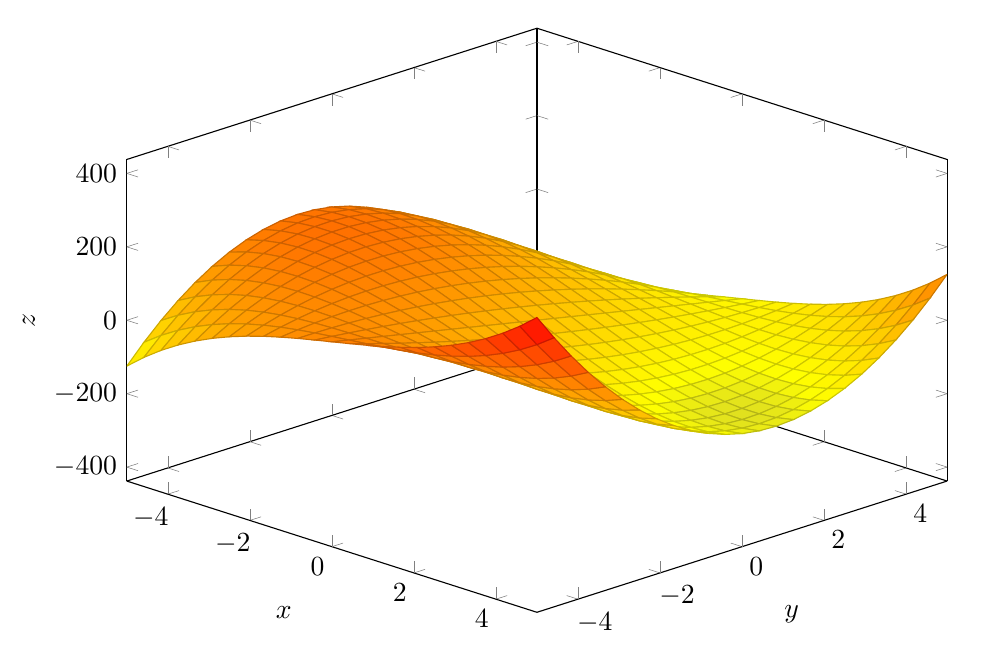
\begin{tikzpicture}
        \begin{axis}[
            width=12cm, height=9cm,
            view={45}{30},
            xlabel={$x$}, ylabel={$y$}, zlabel={$z$},
            xmin=-5, xmax=5,
            ymin=-5, ymax=5,
            ]
            \addplot3[surf]{x^3 + 3*x*y^2 - 51*x - 24*y};            
        \end{axis}
    \end{tikzpicture}

Wykres funkcji $ f(x,y) = x^3 + 3xy^2 - 51x - 24y, \quad -5 \leq x \leq 5, \ -5 \leq y \leq 5 $
\end{center}

\textbf{Wykresy niektórych popularnych funkcji}

\begin{itemize}
    \item $ z = Ax + By + C $ -- płaszczyzna o wektorze normalnym $ \vec{n} = [A, B, -1] $ i przechodząca przez punkt $ (0,0,C) $.
    \item $ z = z_0 + \sqrt{r^2 - (x-x_0)^2 - (y-y_0)^2} $ -- górna półsfera o środku w $(x_0, y_0, z_0)$ i promieniu $r > 0$. Np.
    $ z = 3 + \sqrt{7 - x^2 - (y-1)^2} : \ S(0,1,3), \ r=\sqrt{7} $

    $ z = z_0 - \sqrt{r^2 - (x-x_0)^2 - (y-y_0)^2} $ -- analogiczna półsfera ale dolna.

    Obie pochodzą z równania całej sfery: $ (x - x_0)^2 + (y - y_0)^2 + (z - z_0)^2 = r^2 $.
    \item $ z = z_0 + a\sqrt{(x-x_0)^2 + (y-y_0)^2}, \ a \neq 0 $ -- powierzchnia stożkowa o wierzchołku w $ P = (x_0,y_0,z_0) $
    i osi symetrii równoległej do osi $Z$.

    $a > 0$ -- wierzchołek w dół, $a < 0$ -- wierzchołek w górę.

    $|a| = \tan \alpha $, gdzie $\alpha$ jest kątem między prostą będącą tworzącą stożka

    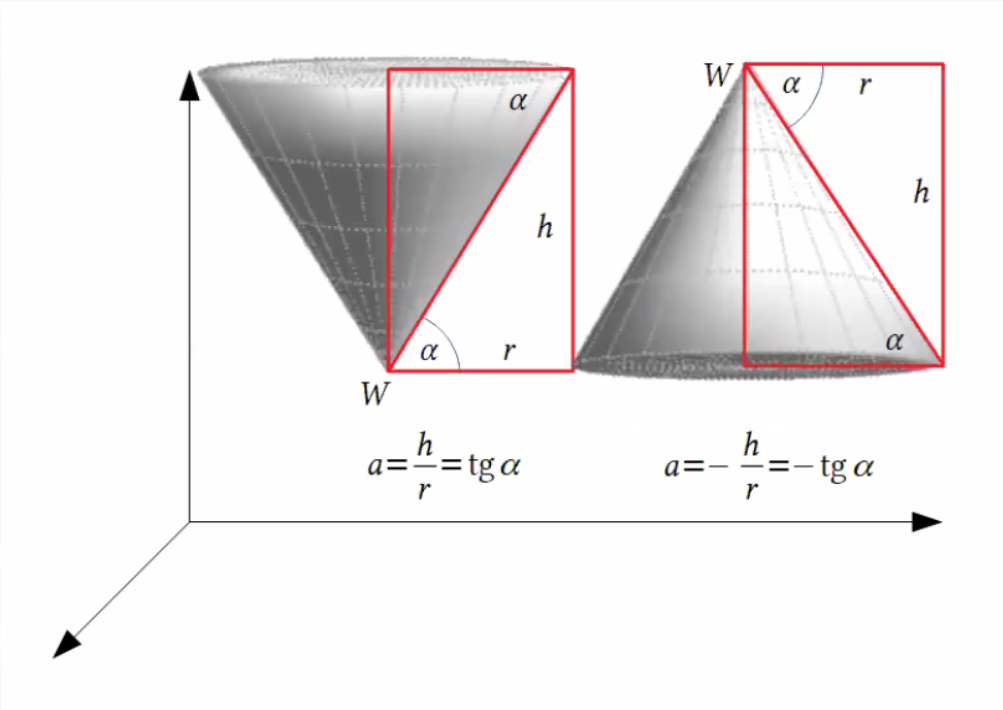
\includegraphics[scale=0.5]{img/stozek_wlzm.png}
\end{itemize}

Powierzchnia stożkowa i półsfera są szczególnymi przypadkami tzw. \underline{powierzchni obrotowych} w $\mathbb{R}^3$. \\

Powierzchnią obrotową w $\mathbb{R}^3$ wokół osi $Z$ będziemy nazywali zbiór wszystkich możliwych punktów
$(x,y,z)$ taki, że podstawienie $r = \sqrt{x^2 + y^2}$ wyznacza zbiór $z$ jako współrzędne wszystkich par $(z,r)$
tworzących pewną krzywą na płaszczyźnie, przy czym zbiór wszystkich $r \geq 0$ jest zbiorem otwartym.

Zatem jeżeli ta powierzchnia jest dana przez pewne równanie postaci
$$ F(x,y,z) = 0 $$
to podstawienie $ r = \sqrt{x^2 + y^2} $ usuwa wszystkie $x$ i $y$ i prowadzi do równania zależnego tylko od $z$ oraz $r$.

W szczególności gdy mamy $z = f(x,y)$ i podstawienie $r$ powoduje, że $f$ zależy tylko od $r$ to wykresem $f$ jest powierzchnia
obrotowa wokół osi $Z$. \\

\begin{tw}{Geometryczne własności takiej powierzchni}

\begin{itemize}
    \item Niepuste przecięcie powierzchni z dowolną płaszczyzną prostopadłą do osi $Z$ jest punktem, okręgiem lub sumą tych zbiorów.
    \item Niepuste przecięcie powierzchni z dowolną płaszczyzną zawierającą oś $Z$ jest krzywą o tym samym kształcie. \\
\end{itemize}

\end{tw}

Na przykład dla powierzchni stożkowej $ z = a\sqrt{x^2 + y^2}, \ a > 0 $, przecięcie płaszczyzną prostopadłą do osi $Z$ jest okręgiem
lub wierzchołkiem, a przecięcie płaszczyzną zawierającą oś $Z$ jest sumą dwóch półprostych wychodzących z wierzchołka.

\begin{center}
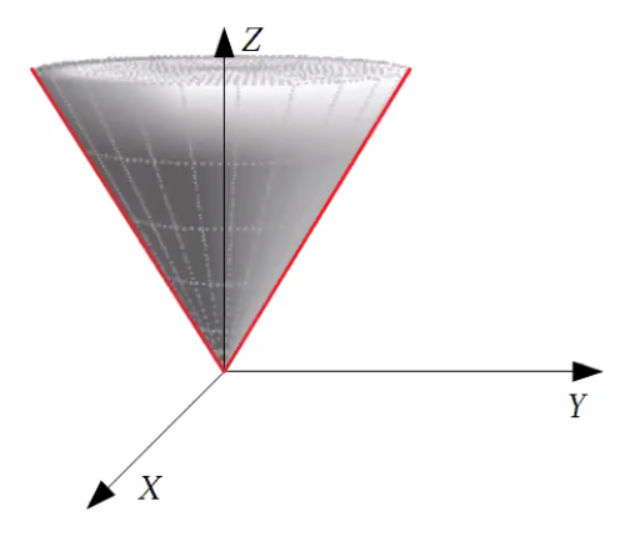
\includegraphics[scale=0.6]{img/stozek_wlzm_2.png}
\end{center}

Sposób rysowania takich powierzchni opiera się na spotstrzeżeniu, że dla $x = 0$ i $y \geq 0$ mamy $ r = \sqrt{y^2} = y \geq 0 $.
Zatem rysujemy w płaszczyźnie $YZ$ wykres odpowiedniej krzywej dla $y \geq 0$, a następnie obracamy go wokół osi $Z$. Tworzy to
żądaną powierzchnię obrotową. \\

Poprzedni przykład raz jeszcze: $ z = a\sqrt{x^2 + y^2}, \ a > 0 $.

Tutaj dla $ r = \sqrt{x^2 + y^2} \geq 0 $ mamy $z =ar$. Zatem biorąc $ r = y \geq 0 $ w płaszczyźnie $YZ$ dostajemy wykres
funkcji liniowej $ z = f(0, y) = ay, \ y \geq 0 $. Jest to półprosta

\begin{center}
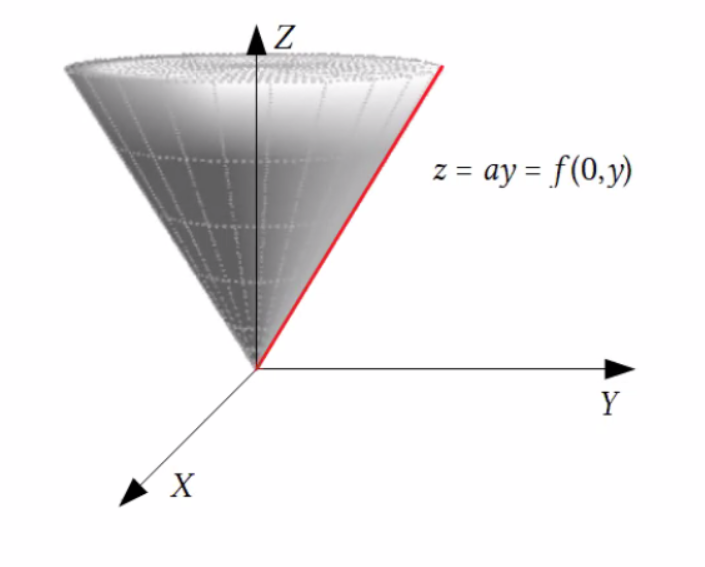
\includegraphics[scale=0.6]{img/stozek_wlzm_3.png}
\end{center}

Rozszerzanie powyższego przypadku -- powierzchnia obrotowa wokół osi równoległej do osi $Z$.

Jeżeli dla pewnych $x_0, y_0 \in \mathbb{R}$ podstawienie $ r = \sqrt{(x - x_0)^2 + (y - y_0)^2} $ usuwa wszystkie $x$ i $y$ i prowadzi
do równania zależnego tylko od $z$ oraz $r$ to dana powierzchnia jest powierzchnią obrotową wokół prostej
$ L : x = x_0, \ y = y_0, \ z\in \mathbb{R} $.

Jest to zatem przypadek powierczhni opisanej poprzednio (czyli dla $x_0 = y_0 = 0$) ale przesunięty następnie o wektor $ \vec{v} = [x_0, y_0, 0] $. \\

\begin{przyklad}
Powierzchnia dana równaniem $ z = (x+2)^2 + (y-1)^2 $
Tutaj mamy $ x_0 = -2 $ oraz $ y_0 = 1 $ i podstawienie $ r = \sqrt{(x+2)^2 + (y-1)^2} $ daje równanie $ z = r^2, \ r \geq 0 $.
Zatem biorąc $ r = y \geq 0 $ w płaszczyźnie $YZ$ dostajemy wykres funkcji $ z = f(0, y) = y^2, \ y \geq 0 $. Jest to prawa gałąź
paraboli.

Obracając ją następnie wokół osi $Z$ dostajemy powierzchnię zwaną paraboloidą.

\begin{center}
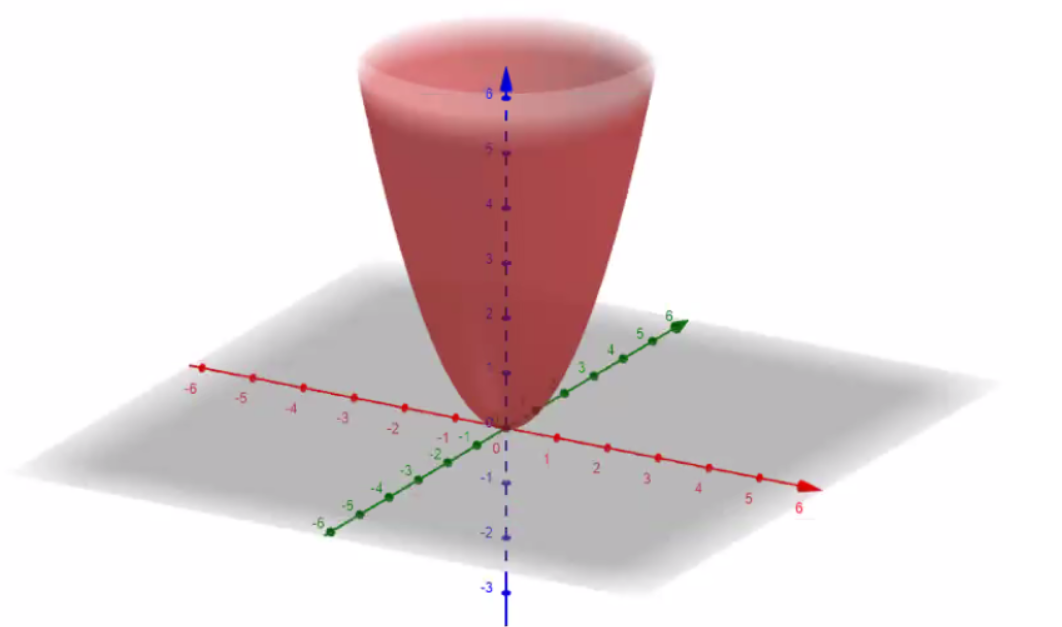
\includegraphics[scale=0.6]{img/paraboloida.png}
\end{center}

Na koniec przesuwamy powyższą powierzchnię o wektor $ \vec{v} = [x_0, y_0, 0] = [-2, 1, 0] $ i to daje naszą powierzchnię.
\end{przyklad}

\subsection{Powierzchnie walcowe}

Powierzchnia jest nazywana powierzchnią walcową równoległą do osi $Z$ jeżeli z faktu, że punkt $ (x_0,y_0,z_0) $
należy do powierzchni wynika, że dla dowolnego $z$ każdy punkt postaci $(x_0, y_0, z_0)$ też należy do tej powierzchni.

To oznacza, że jeżeli taka powierzchnia jest dana przez pewne wyrażenie to równanie to \textbf{nie zawiera} zmiennej $z$.

Geometrycznie -- niepuste przecięcie powierzchni z dowolną płaszczyzną równoległą do osi $Z$ daje krzywą o tym samym kształcie.

Stąd sposób tworzenia wykresów takich powierzchni -- rysujemy w płaszczyźnie $XY$ (czyli dla $z=0$) krzywą zadaną wyjściową relacją,
a potem wykres tej krzywej przesuwamy wzdłuż osi $Z$ i to generuje daną powierzchnię. \\ 

Dwa pozostałe przypadki są analogiczne:

\begin{itemize}
    \item gdy relacja definiująca powierzchnię nie zawiera $x$ to rysujemy odpowiednią krzywą w płaszczyźnie $YZ$
    , a potem jej wykres przesuwamy wzdłuż osi $X$,
    \item gdy relacja definiująca powierzchnię nie zawiera $y$ to rysujemy odpowiednią krzywą w płaszczyźnie $XZ$,
    a potem jej wykres przesuwamy wzdłuż osi $Y$.
\end{itemize}

Stąd prosta reguła -- odpowiednią krzywą przesuwamy zawsze wzdłuż tej osi, która odpowiada zmiennej \textbf{nieobecnej} w równaniu. \\

\begin{przyklad}

Powierzchnia o równaniu $ x^2 + y^2 = 1 $.

Nie występuje $z$, a więc jest to powierzchnia walcowa równoległa do osi $Z$.

Wyznaczamy krzywą daną powyższą relacją w płaszczyźnie $XY$ -- jest to okrąg o środku w układzie współrzędnych i promieniu równym $1$.

Po przesunięciu tego okręgu wzdłuż osi $Z$ zostaje wygenerowana powierzchnia -- jest to powierzchnia boczna walca o nieskończonej długości.
Stąd bierze się nazwa tego typu krzywych.

\begin{center}
    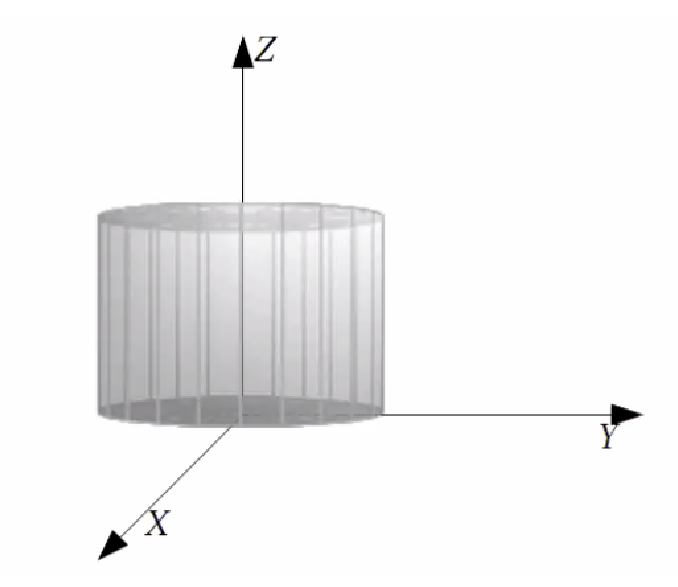
\includegraphics[scale=0.6]{img/walec.png}
\end{center}

\end{przyklad}


\begin{tw}{Definicja}

Poziomica funkcji $ z = f(x,y) $ na wysokości $h$ to zbiór
$$ D_h = \{ (x,y): f(x,y) = h \} $$
Jest to rzut na płaszczyznę $XY$ zbioru -- najczęściej krzywej -- będącego przekrojem wykresu $f$ płaszczyzną o równaniu $z = h$.
\end{tw}

\textbf{Interpretacja geograficzna}

Jeśli płaszczyzna $XY$ jest "mapą" i wyznacza "poziom morza", $z$ -- wysokością nad "poziomem morza", a wykres $f$ jest "rzeźbą terenu"
to poziomica jest krzywą na "mapie" która łączy punkty odpowiadające tej samej "wysokości" $h$.

Na podstawie zagęszczenia poziomic dla odpowiednio dobranych $h$ możemy przewidzieć kształt wykresu $f$ -- czy jest stromy czy płaski.


\subsection{Pochodne cząstkowe pierwszego rzędu funkcji wielu zmiennych}

Są to pochodne danej funkcji liczone względem jednej zmiennej, a pozostałe zmienne są stałe i przyjmują rolę parametrów.

Oznaczenie dla $ f = f(x,y) $:

$$ \dpartial{f}{x} \ \textrm{lub} \ f_x \ \textrm{-- pochodna po} \ x $$
$$ \dpartial{f}{y} \ \textrm{lub} \ f_y \ \textrm{-- pochodna po} \ y $$

Formalna definicja: 
$$ \dpartial{f}{x} (x_0,y_0) = \lim_{h \to 0} \frac{f(x_0 + h, y_0) - \fzero}{h} $$

$$ \dpartial{f}{y} (x_0,y_0) = \lim_{h \to 0} \frac{f(x_0, y_0 + h) - \fzero}{h} $$

Dla funkcji $n$ zmiennych $ f = f(x_1, x_2, ..., x_n) $:
$$ \dpartial{f}{x_i} (x_1, x_2, ..., x_n) = \lim_{h \to 0} \frac{f(x_1, x_2, ..., x_{i - 1}, 
\textcolor{blue}{x_i + h}, x_{i + 1}, ..., x_n) - f(x_1, x_2, ..., \textcolor{blue}{x_i}, ..., x_n)}{h} $$ \\


\subsection{Interpretacja geometryczna dla funkcji 2 zmiennych}

Wykres każdej funkcji $f$ dwóch zmiennych można przeciąć płaszczyzną równoległą do osi $Z$. Powstaje wtedy pewna krzywa, która jest częścią wspólną wykresu $f$
oraz płaszczyzny. Jest to szczególny przypadek tzw. funkcji \underline{warunkowej} o której wkrótce powiemy więcej. \\

Gdy taka krzywa jest regularna to możemy liczyć dla niej pochodną.

Gdy płaszczyzna przekroju przechodzi przez punkt $ P=(x_0, y_0, \fzero) $ to pochodna tej krzywej jest równa

\begin{itemize}
    \item $ \dpartial{f}{x} (x_0, y_0) $, gdy płaszczyzna jest $\parallel XZ $,
    \item $ \dpartial{f}{y} (x_0, y_0) $, gdy płaszczyzna jest $\parallel YZ $. 
\end{itemize}

\begin{center}
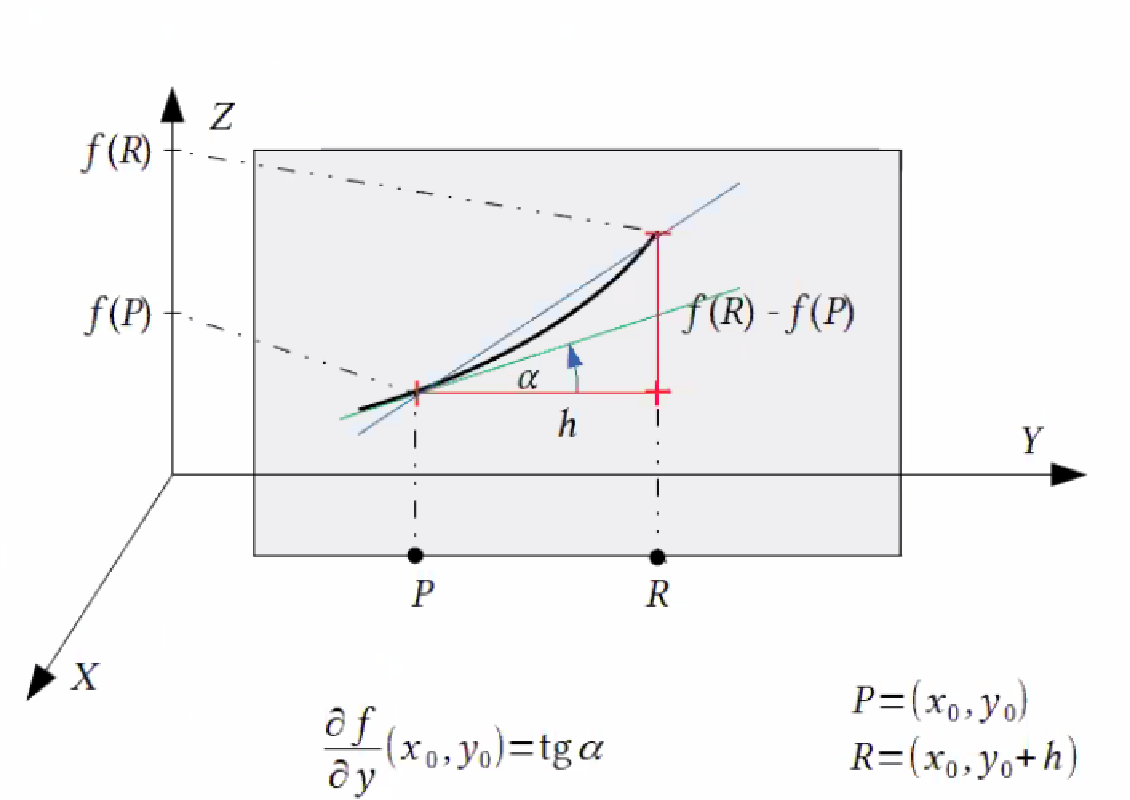
\includegraphics[scale=0.4]{img/interpretacja_geom.png}
\end{center}

\textbf{Sposób wyznaczania pochodnych cząstkowych w praktyce}

Ponieważ tylko jedna zmienna jest w użyciu, a pozostałe stają się parametrami to korzystamy z reguł różniczkowania
funkcji $1$ zmiennej.

Pamiętać należy, że dla wybranej zmiennej dowolne wyrażenie z każdą inną zmienną \textbf{staje się stałą} i jej pochodna
po wybranej zmiennej jest \textbf{równa 0}.

\begin{przyklad}
\[ \dpartial{}{y} (4x^2 + 3 \sin x + 5) = 0, \quad \dpartial{}{x} (ye^{z + 2y}) = 0 \quad \textrm{itd.} \]
\end{przyklad}

\begin{przyklad}

$$ f(x,y) = x \sin (xy^3) $$
Wtedy różniczkując po $x$ mamy pochodną iloczynu:
\[ \dpartial{f}{x} = f_x = (x)_x \cdot \sin(xy^3) + x \cdot (\sin (xy^3))_x = \sin(xy^3) + x \cdot \cos(xy^3) \cdot y^3 \]

Natomiast różniczkując po $y$ mamy mnożenie $\sin (xy^3)$ przez stałą dla $y$ (czyli $x$) i nie trzeba stosować pochodnej iloczynu
\[ \dpartial{f}{y} = f_y = (x \cdot \sin (xy^3))_y = x \cdot (\sin (xy^3))_y = x \cdot \cos(xy^3) \cdot 3y^2x \]
\end{przyklad}


\subsection{Pochodne drugiego rzędu}

Mając pochodne $1$ rzędu definiujemy pochodne drugiego rzędu jako pochodne pierwszego rzędu z pochodnych pierwszego rzędu.
W szczególności, dla $ f = f(x,y) $ mamy $4$ pochodne drugiego rzędu. \\

Pochodne \underline{jednorodne} po danej zmiennej:
\begin{itemize}
    \item $ \frac{\partial^2 f}{\partial x^2} = \dpartial{}{x} \left( \dpartial{f}{x} \right) $ -- dwukrotne różniczkowanie $f$ po $x$,
    \item $ \frac{\partial^2 f}{\partial y^2} = \dpartial{}{y} \left( \dpartial{f}{y} \right) $ -- dwukrotne różniczkowanie $f$ po $y$,
\end{itemize}

Pochodne \underline{mieszane}:

\begin{itemize}
    \item $ \frac{\partial^2 f}{\partial y \partial x} = \dpartial{}{y} \left( \dpartial{f}{x} \right) $ -- różniczkowanie wpierw po $x$, potem po $y$,
    \item $ \frac{\partial^2 f}{\partial x \partial y} = \dpartial{}{x} \left( \dpartial{f}{y} \right) $ -- różniczkowanie wpierw po $y$, potem po $x$, \\
\end{itemize}

Inne oznaczenia to $ f_{xx}, f_{yy}, f_{xy}, f_{yx} $, gdzie indeks dolny oznacza zmienne, po których kolejno różniczkujemy.

W przypadku pochodnych mieszanych $ f_{xy}, f_{yx} $, trzeba ustalić kolejność różniczkowania.

Przyjmujemy naturalną kolejność, wtedy mamy $ f_{xy} = (f_x)_y $ \ oraz \ $ f_{yx} = (f_y)_x $,

co oznacza, że 

$ \frac{\partial^2 f}{\partial y \partial x} = f_{xy} $ \ i \ $ \frac{\partial^2 f}{\partial x \partial y} = f_{yx} $. \\

Dla funkcji $n$ zmiennych $ f = f(x_1, x_2, ..., x_n) $:
$$ \frac{\partial^2 f}{\partial x_j \partial x_i} = \dpartial{}{x_j} \left( \dpartial{f}{x_i} \right) = (f_{x_i})_{x_j} = f_{x_i x_j} $$ \\

\begin{przyklad}

$$ f(x,y) = \frac{2^y}{x+1} $$

$$ \textrm{Tutaj} \quad  f_x = -\frac{2^y}{(x+1)^2}, \ f_y = \frac{2^y \ln 2}{x+1} \quad \textrm{oraz} $$

$$ f_{xx} = (f_x)_x = \left( - \frac{2^y}{(x+1)^2} \right)_x = -2^y \left( \frac{1}{(x+1)^2} \right)_x = 2^y \cdot \frac{2}{(x+1)^3} $$

$$ f_{yy} = (f_y)_y = \left( \frac{2^y \ln 2}{x+1} \right)_y = \frac{\ln2}{x+1} \cdot (2^y)_y = \frac{2^y \cdot (\ln2)^2}{x+1} $$

$$ f_{xy} = (f_x)_y = \left( - \frac{2^y}{(x+1)^2} \right)_y = \left( \frac{-1}{(x+1)^2} \right) \cdot (2^y)_y = - \frac{2^y \ln2}{(x+1)^2} $$

$$ f_{yx} = (f_y)_x = \left( \frac{2^y \ln2}{x+1} \right)_x = 2^y \ln2 \left( \frac{1}{x+1} \right)_x = 2^y \ln2 \left( \frac{-1}{(x+1)^2} \right) = - \frac{2^y \ln2}{(x+1)^2} $$ \\

Otrzymaliśmy $ f_{xy} = f_{yx} $.

Jest to szczególny przypadek znanego twierdzenia.
\end{przyklad}

\begin{tw}{Twierdzenie Schwarza o pochodnych mieszanych}

Gdy pochodne mieszane drugiego rzędu są funkcjami ciągłymi w danym punkcie to są w tym punkcie równe.

W praktyce dla funkcji regularnych warunek ciągłości drugiego rzędu występuje zawsze na całych dziedzinach
stąd prawie zawsze zobaczymy równość wzorów pochodnych mieszanych.
\end{tw}

\begin{tw}{Definicja}
Niech $k \in \mathbb{N}^+$ \ oraz \ $ f = f(x_1, x_2, ..., x_n) $. Pochodna rzędu $k$ funkcji $f$ to funkcja
\[ \frac{\partial^k f}{\partial x_{n_1}... \partial x_{n_2} \partial x_{n_k}} = \dpartial{}{x_{n_k}}
= \left( ... \left( \dpartial{}{x_{n_2}} \left( \dpartial{f}{x_{n_1}} \right) \right) ... \right) = f_{x_{n_1}, x_{n_2}, ..., x_{n_k}} \]

gdzie zmienne \ $ x_{n_1}, x_{n_2}, ..., x_{n_k} $ są dowolnymi ze zmiennych \ $x_1, x_2, ..., x_n$. \bigskip

Oznacza to różniczkowanie funkcji $k$ razy, po kolei po zmiennych
\[ x_{n_1}, x_{n_2}, ..., x_{n_k} \]

\end{tw}

Pochodne jednorodne to te, w których różniczkujemy po tej samej zmiennej $k$ razy, np. $f_{xxx}$.

Pochodne mieszane to te pochodne, w których różniczkujemy przynajmniej po dwóch różnych zmiennych np. $ \frac{\partial^4 f}{\partial x \partial x \partial y \partial x} = f_{xyxx} $

Twierdzenie Schwarza pozostaje prawdziwe dla pochodnych mieszanych rzędu $k$.

\subsection{Płaszczyzna styczna do funkcji dwóch zmiennych}

\begin{tw}{Definicja}
Niech \ $ R = (x,y,z) $ \ oraz \ $ P = (x_0, y_0, z_0) $. Definiujemy zbieżność
\[ R \to P \ \Leftrightarrow \ x \to x_0 \ \land \ y \to y_0 \ \land \ z \to z_0 \]
Nazywamy to zbieżnością po współrzędnych.

\end{tw}

\begin{tw}{Definicja}

Niech teraz $P$ i $R$ należą do wykresu funkcji $f$. 

Czyli 
\[ z = f(x,y), \quad z_0 = \fzero \]
Ponadto niech $ \Pi $ będzie płaszczyzną przechodzącą przez $P$.

$\Pi$ nazywamy \underline{płaszczyzną styczną} do wykresu $f$ w punkcie $P$ jeżeli kąt między prostą $PR$ oraz płaszczyzną $\Pi$ dąży do 0, gdy $R \to P$.

Jest to uogólnienie prostej stycznej do wykresu funkcji jednej zmiennej.
\end{tw}

\begin{tw}{Definicja}
$ f = f(x,y) $ jest funkcją \underline{różniczkowalną} w punkcie \ $(x_0, y_0) \in D_f$, \ gdy istnieje płaszczyzna styczna do wykresu $f$
w punkcie \ $ P = (x_0, y_0, \fzero) $.
\end{tw}

Przykład funkcji nieróżniczkowalnej w pewnym punkcie: powierzchnia stożkowa w wierzchołku (zobacz rysunek powierzchni stożkowych str. 50)

\begin{tw}{Twierdzenie}
Gdy na pewnym kole bez brzegu zawierającym \ $(x_0, y_0) \in D_f $ \ $f$ ma ciągłe pochodne cząstkowe pierwszego rzędu to $f$ jest różniczkowalna w punkcie $(x_0, y_0)$.
\end{tw}

\begin{tw}{Twierdzenie -- wzór na płaszczyznę styczną do $f$}
    Jeżeli $f$ jest różniczkowalna w punkcie $(x_0, y_0)$ to płaszczyzna styczna do wykresu $f$ w $P = (x_0, y_0, \fzero)$ jest dana wzorem
    \[ z - \fzero = f_x(x_0, y_0) \cdot (x - x_0) + f_y(x_0, y_0) \cdot (y - y_0) \]
\end{tw}

Uwagi 
\begin{itemize}
    \item Warunek ciągłości pochodnych na kole jest spełniony dla zdecydowanej większości funkcji elemetnarnych na całej dziedzinie funkcji.
    \item Wzór na płaszczyznę styczną jest analogiczny do wzoru na prostą styczną do funkcji jednej zmiennej.
    \item Płaszczyznę styczną można zapisać w postaci ogólnej
    \[ A(x - x_0) + B(y - y_0) - 1(z - z_0) = 0 \]
    gdzie
    \[ z_0 = \fzero, \quad A = f_x(x_0, y_0), \quad B = f_y(x_0, y_0) \]
    Stąd wektorem normalnym jest
    \[ \vec{n} = [A, B, -1] = [f_x(x_0, y_0), f_y(x_0, y_0), -1] \] 
\end{itemize}

\begin{przykladbig}
    Dana jest funkcja \ $ f(x,y) = x^2 - 2y^2 $

    a) Znaleźć płaszczyznę styczną do wykresu $f$ w punkcie \ $ P = (1, 2, z_0) $.

    b) Znaleźć wszystkie punkty wykresu $f$ w których płaszczyzna styczna jest równoległa do płaszczyzny \ $ \Pi_1: x - 2y + 2z + 5 = 0 $
    \bigskip

    a) $ \Pi_s $ w $ P = (1, 2, z_0)$

    $ z_0 = f(1,2) = -7 $

    \[ \begin{array}{lll}
        f_x = 2x && A = f_x(1,2) = 2 \\
        f_y = -4y && B = f_y(1,2) = -8
    \end{array} \]

    Wzór 
    \[ z - (-7) = 2(x-1) - 8(x-2) \quad \text{lub} \quad \ 2(x-1) - 8(y-2) - (z+7) = 0 \]

    b)
    \[ \Pi_s \ \| \ \Pi : x - 2y + 2z + 5 = 0 \]
    \[ \vec{n} = [1,-2,2] \ \bot \ \Pi \]
    \[ \vec{n_s} = [f_x, f_y, -1] \ \bot \ \Pi_s \]

    \[ \Pi \ \| \ \Pi_s \ \Leftrightarrow \ \vec{n} \ \| \ \vec{n_s} \ \Leftrightarrow \ \frac{f_x}{1} = \frac{f_y}{-2} = \frac{-1}{2} \]

    Trzeba zatem rozwiązać układ równań
    \[ \begin{cases}
        f_x = -\frac{1}{2} = 2x \\
        f_y = 1 = -4y
    \end{cases} \]

    Rozwiązanie to
    \[ x = x_0 = -\frac{1}{4} \]
    \[ y = y_0 = -\frac{1}{4} \]

    Stąd
    \[ z_0 = f\left(-\frac{1}{4}, -\frac{1}{4}\right) = -\frac{1}{16} \]
    I punkt to jest
    \[ P = \left(-\frac{1}{4}, -\frac{1}{4}, -\frac{1}{16}\right) \]
\end{przykladbig}

Bezpośrednie zastosowanie: \underline{przybliżanie funkcji płaszczyzą styczną}

Równanie płaszczyzny stycznej $\Pi$ do wykresu $f$ w $P = (x_0, y_0, \fzero)$ można zapisać wzorem

\[ z = \fzero + f_x(x_0, y_0) \cdot (x - x_0) + f_y(x_0, y_0) \cdot (y - y_0) \]

Gdy teraz \ $ R = (x, y, f(x,y)), \ Q = (x,y,z) \in \Pi $ \ i \ $ x \approx x_0 $ oraz \ $ y \approx y_0 $ to 
\ $ R \approx P \approx Q $, \ a więc \ $ R \approx Q $ \ i \ $ z \approx f(x,y) $.

To daje wzór na przybliżoną wartość \ $f(x,y)$:

\[ f(x,y) \approx f(x_0,y_0) + f_x(x_0, y_0) \cdot (x - x_0 ) + f_y(x_0, y_0) \cdot (y - y_0) \]

Zastosowanie:
\begin{itemize}
    \item $ x_0, y_0 $ -- "ładne": łatwe do obliczenia,
    \item $ x,y $ -- to co mamy w zadaniu.
\end{itemize}

\begin{przyklad}
    Obliczyć w przybliżeniu i bez kalkulatora $ (2,005)^5 \ln(0,98) $ \medskip

    Mamy \ $ (2,005)^5 \ln(0,98) = f(2.005, 0.98) $.

    Zatem
    \[ f(x,y) = x^5 \ln y, \ x = 2,005, \ y = 0,98 \]

    Bierzemy \ $x_0 = 2$ \ oraz \ $ y_0 = 1 $.

    To daje
    \[ f_x = 5x^4 \ln y, \quad f_y = \frac{x^5}{y}, \quad f_x(2,1) = 0, \quad f_y(2,1) = 32 \quad \text{oraz} \quad f(2,1) = 0 \]

    Zatem
    \[ (2,005)^5 \ln (0,98) \approx 0 + 0 \cdot (2,005 - 2) + 32 \cdot(0,98 - 1) = -0,64 \]

    Dokładna wartość: $ -0,65461 $. Błąd wynosi ok. 0,015 czyli 2,34\%.
\end{przyklad}

Dalsze zastosowanie wzoru

Biorąc \ $ x - x_0 = \Delta x, \quad y - y_0 = \Delta y $ \ mamy \ $ x = \Delta x + x_0, \quad y = \Delta y + y_0 $.
\medskip

To daje wzór
\[ f(x_0 + \Delta x, y_0 + \Delta y) \approx \fzero + f_x(x_0, y_0) \cdot \Delta x + f_y(x_0, y_0) \cdot \Delta y \]
Czyli
\[ f(x_0 + \Delta x, y_0 + \Delta y) - \fzero \approx f_x(x_0, y_0) \cdot \Delta x + f_y(x_0, y_0) \cdot \Delta y \]

Oznaczając przez $ \Delta f $ "błąd bezwzględny funkcji" mamy
\[ \Delta f  = | f(x_0 + \Delta x ,y_0 + \Delta y) - \fzero | \ \approx f_x(x_0, y_0) \cdot \Delta x + f_y(x_0, y_0) \cdot \Delta y \]

Gdy oba iloczyny pod modułem z prawej strony mają ten sam znak błędy kumulują się i mamy
\[ \Delta f \approx | f_x(x_0, y_0) | \ \cdot \ | \Delta x | \ + \ | f_y(x_0, y_0) | \ \cdot \ | \Delta y | \]

To jest wzór na tzw. \underline{różniczkę zupełną}.

Jest to uogólnienie wzoru z AM1 dla funkcji jednej zmiennej \ $ f = f(x) $:
\[ \Delta f \approx | f'(x_0) | \ \cdot \ | \Delta x | \]

Zastosowania -- przy pomiarach z błędem

Mierzymy $x$ z dokładnością $ | \Delta x| \approx 0 $.

Wówczas błąd bezwzględny pomiaru $f$ wynosi w przybliżeniu $ \Delta f $.

\begin{przyklad}
    W obwodzie zmierzono wartość prądu stałego \ $ I = 3 \ A \pm 0,1 \ A $ oraz rezystancję \ $ R = 2 \ \Omega \pm 0,01 \Omega $.

    Z jaką w przybliżeniu dokładnością zmierzymy wydzieloną moc? \bigskip

    Mamy
    \[ P = P(I, R) = I^2 R, \quad I_0 = 3, \quad R_0 = 2, \quad, \Delta I = \pm 0,1, \quad \Delta R = \pm 0,01 \]

    Czyli
    \[ P_I = 2 IR, \quad P_R = I^2, \quad P_I(3,2) = 12, \quad P_R(3,2) = 9 \]
    A więc
    \[ \Delta P = |12| \ \cdot 0,1 + |9| \ \cdot 0,01 = 1,29 [\textrm{W}] \]
\end{przyklad}


\subsection{Pochodna kierunkowa}

\begin{tw}{Definicja}
    Dla funkcji 2 zmiennych \ $ f = f(x,y) $ \ pochodna ta mierzy zmienność $f$ w zadanym kierunku \ $ \vec{v} = [a,b] $.

    Geometrycznie, jest to wersja pochodnej jednostronnej krzywej, która jest częścią wspólną wykresu $f$ oraz płaszczyzny równoległej
    do osi $Z$ i do wektora $\vec{v}$.

    Oznaczenie :
    \[ \dpartial{f}{\vec{v}}(x,y) \quad \text{lub} \quad f_{\vec{v}}(x,y) \]
\end{tw}

\textbf{Uwaga! Do definicji będziemy zawsze używać wektorów jednostkowych:}
\[ |\vec{v}| = 1 \]

\begin{tw}{Ogólna definicja dla funkcji $n$ zmiennych}
    Ustalamy punkt $P$ w $\mathbb{R}^n$ i rozpatrujemy półprostą o początku w $P$ i o kierunku zgodnym z $\vec{v}$ czyli zbiór tych punktów
    $R$ dla których $\overrightarrow{PR}$ i $\vec{v}$ mają zgodne kierunki.

    Badamy proporcję różnicy wartości $f$ w punktach $R$ i $P$ do odległości $R$ od $P$ przy przejściu granicznym $ R \to P $.

    Daje to definicję
    \[ \dpartial{f}{\vec{v}}(P) = \lim_{R \to P} \frac{f(R) - f(P)}{|\overrightarrow{PR}|} \]

    \begin{center}
        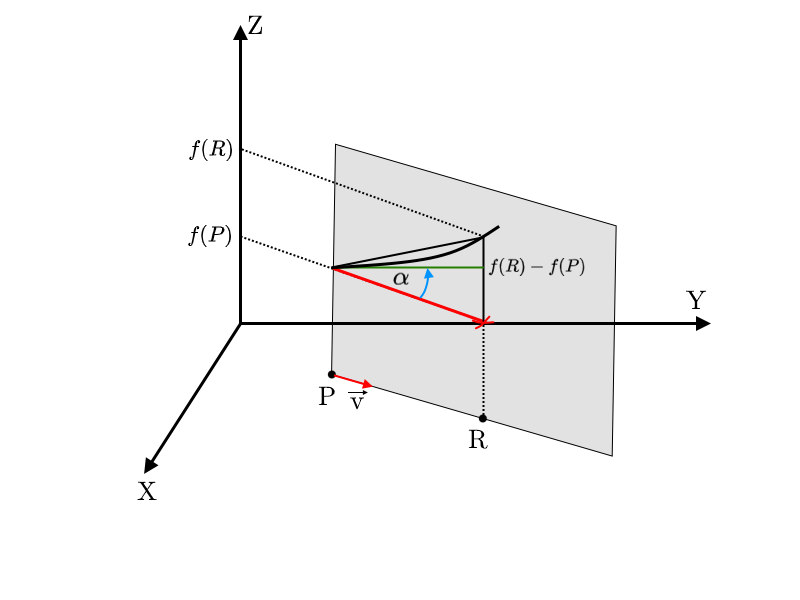
\includegraphics[scale=0.5]{img/pochodnakierunkowa.png}
    \end{center}
    \[ \dpartial{f}{\vec{v}}(P) = \tan \alpha \]
\end{tw}

W przypadku funkcji 2 zmiennych dla \ $ P = (x_0, y_0) $ \ i \ $ \vec{v} = [a,b] $ \ równanie parametryczne powyższej półprostej ma postać
\[ \begin{cases} 
    x = x_0 + at \\
    y = y_0 + bt
\end{cases} \quad \text{dla} \ t > 0 \]

To oznacza, że
\[ R = (x,y) = (x_0 + at, y_0 + bt) \quad \text{oraz} \quad \overrightarrow{PR} = t \cdot \vec{v} \]
A stąd
\[ |\overrightarrow{PR}| = |t \cdot \vec{v}| = |t| \cdot |\vec{v}| = t \cdot 1 = t \]

Ponieważ \ $ R \to P \ \Leftrightarrow \ t \to 0^+ $ \ oznacza, że
\[ \lim_{R \to P} \frac{f(R) - f(P)}{|\overrightarrow{PR}|} = \lim_{t \to 0^+} \frac{f(x_0 + at, y_0 + bt) - \fzero}{t} \]
a to daje równoważną definicję pochodnej kierunkowej:
\[ \dpartial{f}{\vec{v}} (x_0, y_0) = \lim_{t \to 0^+} \frac{f(x_0 + at, y_0 + bt) - \fzero}{t}, \quad \text{gdzie} \ \vec{v} = [a,b], \ |\vec{v}| = 1 \]

\begin{przyklad}
    Dla \ $ f(x,y) = |x| + 3|y| $ \ i \ $ \vec{v} = \left[ -\frac{\sqrt{2}}{2}, \frac{\sqrt{2}}{2} \right] $ \ mamy w punkcie (0,1)
    \[ \dpartial{f}{\vec{v}} (0,1) = \lim_{t \to 0^+} \frac{f \left( 0 - \frac{\sqrt{2}}{2}t, 1 + \frac{\sqrt{2}}{2}t \right) - f(0,1)}{t}
    = \lim_{t \to 0^+} \frac{ \left| -\frac{\sqrt{2}}{2}t \right| + 3 \left| 1 + \frac{\sqrt{2}}{2}t \right| - 3 }{t} = \]
    \[ \lim_{t \to 0^+} \frac{ \frac{\sqrt{2}}{2}t + 3 \left( 1 + \frac{\sqrt{2}}{2}t \right) - 3 }{t} = \lim_{t \to 0^+} \frac{4 \cdot \frac{\sqrt{2}}{2}t}{t} = 2 \sqrt{2} \]
\end{przyklad}

Z definicji liczymy tylko dla funkcji mało regularnych. Gdy pochodne cząstkowe $f$ są ciągle to mamy lepszy wzór z użyciem \underline{gradientu}.

\subsection{Gradient}

\begin{tw}{Definicja}
    Gradient funkcji w danym punkcie -- wektor pochodnych cząstkowych pierwszego rzędu funkcji $f$ w danym punkcie.

    Oznaczenie: $ \text{grad}\, f$ \ lub \ $ \nabla f $.

    Dla funkcji 2 zmiennych i punktu $ P = (x_0, y_0) $
    \[ \text{grad}\, \fzero = [f_x(x_0, y_0), f_y(x_0, y_0)] \]

    Dla funkcji $n$ zmiennych \ $ f = f(x_1, x_2, ..., x_n) $ \ i punktu \ $ P = (a_1, a_2, ..., a_n) \in \mathbb{R}^n $
    \[ \text{grad} \, f(P) = [f_{x_1}(P), f_{x_2}(P), ..., f_{x_n}(P)] \]
\end{tw}

\begin{tw}{Twierdzenie}
    Gdy pochodne cząstkowe $f$ są ciągłe w \ $ (x_0, y_0) $ \ i \ $ \vec{v} = [a,b] $ \ oraz \ $ |\vec{v}| = 1 $ \ to
    \[ \dpartial{f}{\vec{v}} (x_0, y_0) = \vec{v} \circ (\text{grad} \, \fzero) = a \cdot f_x(x_0, y_0) + b \cdot f_y(x_0, y_0) \]
    Wzór rozszerza się do funkcji większej ilości zmiennych.    
\end{tw}

\begin{przyklad}
    \[ f(x,y) = x^2 \cdot y^3, \quad \vec{v} =\left[ -\frac{1}{2}, \frac{\sqrt{3}}{2} \right] \]
    Obliczyć $ f_{\vec{v}} (-1, 1) $. \bigskip

    Mamy
    \[ f_x = 2xy^3, \quad f_y = 3x^2 y^2 \]
    \[ f_x(-1, 1) = -2, \quad f_y(-1, 1) = 3, \quad \text{grad}\, f(-1, 1) = [-2, 3] \]
    \[ f_{\vec{v}} = [-2, 3] \circ \left[ -\frac{1}{2}, \frac{\sqrt{3}}{2} \right] = 1 + \frac{3 \sqrt{3}}{2} \]
\end{przyklad}

Dalej,
\[ \vec{v} \circ \text{grad}\, \fzero = 1 \cdot | \text{grad}\ \fzero | \cdot \cos \alpha \]
gdzie $\alpha$ jest kątem między tymi dwoma wektorami.

To daje następujące wnioski:

\begin{tw}{Twierdzenie}
    Gdy \ $ \text{grad} \, \fzero = \vec{0} $
    \quad to \quad
    $ \dpartial{f}{\vec{v}} (x_0, y_0) = 0 $
    \quad dla dowolnego $ \vec{v} $.
\end{tw}

\begin{tw}{Twierdzenie}
    $ \dpartial{f}{\vec{v}} (x_0, y_0) $ ma wartość największą kiedy $\vec{v}$ i grad $\ \fzero $ mają zgodne kierunki.

    Ta największa wartość to \ $ | \text{grad}\, \fzero | $.
\end{tw}

\begin{tw}{Twierdzenie}
    $ \dpartial{f}{\vec{v}} (x_0, y_0) $ ma wartość najmniejszą kiedy $\vec{v}$ i grad $\ \fzero $ mają przeciwne kierunki.

    Ta najmniejsza wartość to \ $ -| \text{grad}\, \fzero | $.
\end{tw}

\begin{tw}{Twierdzenie}
    $ \dpartial{f}{\vec{v}} (x_0, y_0) = 0 $ \quad dla \quad $ \text{grad} \, \fzero \neq \vec{0} $
    \quad kiedy \quad
    $ \text{grad} \, \fzero \perp \vec{v} $
\end{tw}

\begin{tw}{Twierdzenie}
    Zbiór wartości \ $ \dpartial{f}{\vec{v}} (x_0, y_0) $ \ w zależności od $\vec{v}$ to przedział
    \[ [ -|\text{grad} \, \fzero|, |\text{grad} \, \fzero | ] \]
    Skrajne wartości są osiągane dla dokładnie jednego wektora (zob. punkty 2 i 3), a pozostałe -- dla dokładnie dwóch wektorów $\vec{v}$.
\end{tw}

\begin{przyklad}
    Dana jest funkcja \ \[ f(x,y) = (x^2 + y^2)e^{x-y} \]

    1.Znaleźć wszystkie wersory $\vec{v}$ dla których \ $ f_{\vec{v}} (-1, 1) $
    
    a) jest największa

    b) jest najmniejsza \medskip

    2. Wyznaczyć zbiór wszystkich punktów (x,y) dla których pochodna kierunkowa w kierunku wersora \ $ \vec{v} = \left[ \frac{3}{5}, \frac{4}{5} \right] $ \ jest równa 0.
    \bigskip

    Wprowadzić wektor $ \vec{v} = [a,b] $ \ co daje
    \[ f_{\vec{v}} (-1, 1) = [a,b] \circ [3e^{-3}, -e^{-3}] = 3e^{-3} a - e^{-3}b \]
    Następnie trzeba analizować tę funkcję \textbf{nie zapominając o dodatkowym warunku}
    \[ \vec{v} = 1 \ \Leftrightarrow \ a^2 + b^2 = 1 \]
    Prowadzi to do układu równań, jest dłuższe i bardziej skomplikowane

    W części 2 potrzebna jest metoda analityczna.
    
    Korzystając ze wzoru na gradient z części a) Mamy
    \[ f_{\vec{v}} = (x,y) = grad\, f(x,y) \circ \vec{v} = [e^{x-y} (2x + x^2 + y^2), e^{x-y}(2y - x^2 - y^2)] \circ \left[ \frac{3}{5}, \frac{4}{5} \right] = \]
    \[ \frac{3}{5} e^{x-y} (2x + x^2 + y^2) + \frac{4}{5} e^{x-y} (2y - x^2 - y^2) = \frac{1}{5} e^{x-y} (6x + 8y - x^2 - y^2) = 0 \]

    To oznacza, że \ $ 6x + 8y - x^2 - y^2 = 0 $

    Jest to równanie okręgu -- po sprowadzeniu do postaci kanonicznej mamy \bigskip

    \textbf{Ciąg dalszy nastąpi po wykładzie w dniu 8.05.2023}
\end{przyklad}

\subsection{Zbieżność w $\mathbb{R}^k$ i granice funkcji wielu zmiennych}

Rozpatrujemy ciąg wielu punktów $ P_n = (x_n, y_n) \in \mathbb{R}^2 $.

Równoważnie możemy myśleć o wektorach $ \vec{v} \in \mathbb{R}^2 $ biorąc wektory pozycyjne punktów $P_n$ czyli $\vec{v} = \vec{OP}_n$.

Niech teraz $ P_0 = (x_0, y_0) \in \mathbb{R}^2 $. Mówimy, że $ P_n \to P_0 $, gdy odległość między $P_n$ i $P_0$ zbiega $0$.

Formalnie
$$ \limn P_n = P_0 \ \Leftrightarrow \ \limn |\overrightarrow{P_0 P_n}| = 0
\ \Leftrightarrow \ \limn \sqrt{(x_n - x_0)^2 + (y_n - y_0)^2} = 0 $$

Podobnie, gdy
$$ P_n = (x_n, y_n, z_n) \in \mathbb{R}^3 \quad \textrm{i} \quad P_0 = (x_0, y_0, z_0) \in \mathbb{R}^3 $$

To definiujemy
$$ \limn P_n = P_0 \ \Leftrightarrow \ \limn |\overrightarrow{P_0 P_n}| = 0
\ \Leftrightarrow \ \limn \sqrt{(x_n - x_0)^2 + (y_n - y_0)^2 + (z_n - z_0)^2} = 0 $$

Analogicznie rozszerzamy tę definicję na przypadek $k$ -- wymiarowy. \\

Poniższe twierdzenie pokazuje, że zbieżność $ P_n \to P_0 $ może być zdefiniowana w równoważny sposób. \\

\begin{tw}{Twierdzenie -- zbieżność po współrzędnych }

Gdy
\[ P_n = (x_n, y_n) \in \mathbb{R}^2 \quad \textrm{i} \quad P_0 = (x_0, y_0) \in \mathbb{R}^2 \]
to mamy równoważność
\[ \limn P_n = P_0 \ \Leftrightarrow \ \limn x_n = x_0 \ \land \ \limn y_n = y_0 \]
\end{tw}

Dowód 

Implikacja $ \Leftarrow $ wynika bezpośrednio z arytmetyki granic :

Jeżeli $ \limn x_n = x_0 \ \land \ \limn y_n = y_0 $ to
$$ \limn |\overrightarrow{P_0 P_n}| = \limn \sqrt{(x_n - x_0)^2 + (y_n - y_0)^2} = \sqrt{(x_n - x_0)^2 + (y_n - y_0)^2} = 0 $$

Zatem
$$ \limn P_n = P_0 $$ \\

Implikacja $ \Rightarrow $ wynika z kolei z twierdzenia o 3 funkcjach. 

Mamy bowiem
$$ 0 \leq |x_n - x_0| = \sqrt{(x_n - x_0)^2} \leq \sqrt{(x_n - x_0)^2 + (y_n - y_0)^2} = |\overrightarrow{P_0 P_n}| $$

Teraz, gdy $ \limn P_n = P_0 \quad \textrm{to} \quad \limn |\overrightarrow{P_0 P_n}| = 0 $
i z twierdzenia o 3 ciągach dostajemy $ \limn |x_n - x_0| = 0 $ a to daje
$ \limn (x_n - x_0) = 0 \ \Leftrightarrow \ \limn x_n = x_0 $

Analogicznie otrzymujemy $ \limn y_n = y_0 $ \\

Jak łatwo zauważyć, twierdzenie ma analogiczną postać w przypadku wyższych wymiarów. \\

\begin{tw}{Definicja -- granica funkcji dwóch zmiennych w punkcie}

$ \lim_{(x,y) \to (x_0,y_0)} f(x,y) = L \ \Leftrightarrow $ dla dowolnych ciągów punktów $ (x_n, y_n) \neq (x_0, y_0) $
i takich, że $ \limn (x_n, y_n) = (x_0, y_0) $ zachodzi równość $ \limn f(x_n, y_n) = L $. \\

Definicja jest analogiczna w przypadku funkcji większej ilości zmiennych.

Równoważny zapis tej granicy, zgodny ze znaczeniem twierdzenia o zbieżności po współrzędnych to
$$ \lim_{\substack{x \to x_0 \\ y \to y_0}} f(x,y) = L $$

Twierdzenie o granicach znane dla funkcji jednej zmiennej (arytmetyka granic, symbole nieoznaczone itd.) pozostają prawdziwe.
\end{tw}

Główny problem -- nie da się bezpośrednio zastosować niektórych popularnych technik, np. reguły de l'Hospitala.

\subsection{Popularne techniki liczenia granic funkcji wielu zmiennych}

\begin{enumerate}
    \item Twierdzenie o 3 funkcjach. Jeżeli dla wszystkich punktów $ P \in \mathbb{R}^k $ z pewnego sąsiedztwa punktu
    $ P_0 \in \mathbb{R}^k $ zachodzi nierówność 
    $$ d(P) \leq f(P) \leq g(P) \quad \textrm{i} \quad \lim_{P \to P_0} d(P) = \lim_{P \to P_0} g(P) = L \quad \textrm{to} \quad \lim_{P \to P_0} f(P) = L $$

    \item Sprowadzenie granicy do przypadku jednej zmiennej.
    
    Jeżeli istnieje nowa zmienna $ t = t(P) $ takie, że $ f(P) = g(t) $ oraz 
    $ \lim_{P \to P_0} t = t_0 $ \ i \linebreak \ $ \lim_{t \to t_0} g(t) = L $ \ to \ $ \lim_{P \to P_0} f(P) = L $ 

    \item \textbf{COŚ O BRAKU GRANICY XD}
    $ \lim_{P \to P_0} f(P) $ nie istnieje
\end{enumerate}

Przypadek 3 jest szczególnie częsty, gdy pojawia się symbol nieoznaczony.

W przypadku funkcji dwóch zmiennych najczęściej wybiera się ciągi punktów $P_n$ i $Q_n$ z dwóch różnych krzywych.

$P$ jest wtedy z wykresu jakiejś krzywej: $ y=g(x)$ \ lub \ $x=g(y)$.

$Q$ jest z wykresu innej krzywej: $y=h(x)$ \ lub \ $x=h(y)$.

Obie krzywe muszą spotykać się w punkcie granicznym $P_0$.

Wtedy granice \ $ \lim_{P \to P_0} f(P) $ \quad i \quad $ \lim_{Q \to P_0} f(Q) $ \ stają się granicami funkcji jednej zmiennej. \\

\begin{przyklad}

$$ \lim_{\substack{x \to 0 \\ y \to 0}} (x^2 + 4y^2) \cos \left( x - 5y + \frac{2}{x} \right) $$

Wiemy, że \ $ x^2 + 4y^2 \geq 0 $ \ oraz \ $ -1 \leq \cos \left( x - 5y \frac{2}{x} \right) \leq 1 $, \ a stąd
$$ -(x^2 + 4y^2) \leq (x^2 + 4y^2) \cos \left( x - 5y + \frac{2}{x} \right) \leq x^2 + 4y^2 $$

Ponieważ 
$$ \lim_{\substack{x \to 0 \\ y \to 0}} (x^2 + 4y^2) = 0 = \lim_{\substack{x \to 0 \\ y \to 0}} (-(x^2 + 4y^2)) $$
z twiedzenia o 3 ciągach otrzymujemy
$$ \lim_{\substack{x \to 0 \\ y \to 0}} (x^2 + 4y^2) \cos \left( x - 5y + \frac{2}{x} \right) = 0 $$ \\

$$ \lim_{\substack{x \to 1 \\ y \to 1 \\ z \to 0}} \frac{2x - y + z - 1 - \ln(2x - y + z)}{(2x - y + z - 1)^2} $$

Tutaj możemy podstawić $ t = 2x - y + z $. Wtedy $ \lim_{\substack{x \to 1 \\ y \to 1 \\ z \to 0}} t = 1 $

i mamy

$$ \lim_{\substack{x \to 1 \\ y \to 1 \\ z \to 0}} \frac{2x - y + z - 1 - \ln(2x - y + z)}{(2x - y + z - 1)^2}
= \lim_{t \to 1} \frac{t - 1 - \ln t}{(t-1)^2} \left[ \frac{0}{0} \right] \stackrel{[H]}{=} \frac{1}{2}$$
\end{przyklad}

\begin{przyklad}

$$ \lim_{\substack{x \to 0 \\ y \to 0}} \frac{\tan (x^2 - y^2)}{x - y} $$

Tutaj znów jest granica typu $ \frac{0}{0} $. Po podstawieniu \ $ t = x^2 - y^2 $ \ mamy granicę podstawową
$ \lim_{t \to 0} \frac{\tan t}{t} = 1 $.

Stąd wniosek, że trzeba nasze wyrażenie rozbić na iloczyn: 
$ \lim_{\substack{x \to 0 \\ y \to 0}} \frac{\tan (x^2 - y^2)}{x^2 - y^2} \cdot \frac{x^2 - y^2}{x - y} $

Mamy wtedy
$$ \lim_{\substack{x \to 0 \\ y \to 0}} \frac{\tan (x^2 - y^2)}{x^2 - y^2} = \lim_{t \to 0} \frac{\tan t}{t} = 1 $$
Oraz
$$ \lim_{\substack{x \to 0 \\ y \to 0}} \frac{x^2 - y^2}{x - y} = \lim_{\substack{x \to 0 \\ y \to 0}} \frac{(x - y)(x + y)}{x - y}
= \lim_{\substack{x \to 0 \\ y \to 0}} (x + y) = 0 $$

Stąd 
$$ \lim_{\substack{x \to 0 \\ y \to 0}} \frac{\tan (x^2 - y^2)}{x - y} = 1 \cdot 0 = 0 $$
\end{przyklad}

\begin{przyklad}

$$ \lim_{\substack{x \to 0 \\ y \to 0}} \frac{x}{y} $$

Tutaj wykażemy brak granicy

Rozpatrujemy 2 krzywe przechodzące przez $(0,0)$. Na przykład \ $ y = x $ \ oraz \ $ y = 2x $.

Biorąc \ $ y = x $ \ mamy
$$ \lim_{\substack{x \to 0 \\ y \to 0}} \frac{x}{y} = \lim_{x \to 0} \frac{x}{x} = 1 $$
Natomiast dla \ $ y = 2x $ mamy
$$ \lim_{\substack{x \to 0 \\ y \to 0}} \frac{x}{y} = \lim_{x \to 0} \frac{x}{2x} = \frac{1}{2} \neq 1 $$
Zatem granica nie istnieje
\end{przyklad}

\subsection{Ciągłość funkcji wielu zmiennych}

Definicja jest analogiczna jak dla funkcji jednej zmiennej -- granica funkcji jest równa wartości.

Formalnie,

$f$ jest ciągła w punkcie $ P_0 \in D_f $, \ gdy \ $ \lim_{P \to P_0} f(P) = f(P_0) $,

$f$ jest ciągła na zbiorze $ A \subset D_f $ jeżeli jest ciągła we wszystkich punktach z $A$. \\

Twierdzenia dotyczące arytmetyki funkcji ciągłych są analogiczne jak w przypadku jednej zmiennej. \\

\begin{przyklad}

Wyznaczyć zbiór punktów ciągłości funkcji

$$ f(x,y) = \left\{ \begin{aligned} 2x + y + 1, & \ x \geq 0 \\ 2y + x, & \ x < 0 \end{aligned} \right. $$

Tutaj rozpatrujemy dwa obszary -- dane warunkami $ x \geq 0 $ \ oraz \ $x < 0$.

Brzegiem obu obszarów jest prosta $ x = 0 $ (oś $Y$).

W punktach \ $ (x,y), \ x > 0 $, \ funkcja jest ciągła, bo jest równa elementarnej na zbiorze otwartym.

Podobnie dla $ x < 0 $..

Pozostaje zbadać ciągłość w punktach brzegowych czyli w $ P_0  = (0, y_0) $.

Ze względu na warunek definiujący zbiór, dla takich punktów zbieżności trzeba rozpatrzeć 2 możliwe typy punktów
$$ P = (x,y) \to P_0 \quad \textrm{dla} \quad x \geq 0 \ \textrm{oraz} \ x < 0 $$

Dla \ $ x \geq 0 $ \ mamy
$$ \lim_{\substack{x \to 0 \\ y \to y_0}} f(x,y) = \lim_{\substack{x \to 0 \\ y \to y_0}} (2x + y - 1) = y_0 - 1 $$

Dla \ $ x < 0 $ \ mamy
$$ \lim_{\substack{x \to 0 \\ y \to y_0}} f(x,y) = \lim_{\substack{x \to 0 \\ y \to y_0}} (2y + x) = 2y_0 $$

Ponadto $ f(0,y_0) = y_0 - 1 $

Stąd ciągłość w \ $ P_0 = (0,y_0) $ \ ma miejsce, gdy \ $ y_0 - 1 = 2y_0 $, \ a więc dla \ $ y_0 = -1$.

Wtedy dla dowolnego ciągu punktów \ $ P = (x,y) \to (0, -1) $ \ mamy
$$ \lim_{\substack{x \to 0 \\ y \to -1}} f(x,y) = f(0,-1) = -2 $$

Zatem zbiorem punktów ciągłości $f$ jest zbiór
$$ D = \{ (x,y) : x \neq 0 \} \cup \{ (0,-1) \} $$

Interpretacja geometryczna wykresu -- składa się z dwóch osobnych ukośnych półpłaszczyzn, które spotykają
się w punkcie $(0, -1) $.
\end{przyklad}


\subsection{Ekstrema funkcji dwóch zmiennych}

\begin{tw}{Definicja}

$f$ ma w $ P = (x_0, y_0) \in D_f $ minimum lokalne gdy $ \fzero $ jest najmniejszą wartością $f$ na pewnym kole o środku w $P$ tzn.
\[ \forall(x,y) \in K \ f(x,y) > f(x_0, y_0) \]

$f$ ma w $ P = (x_0, y_0) \in D_f $ maksimum lokalne gdy $ \fzero $ jest największą wartością $f$ na pewnym kole o środku w $P$ tzn.
\[ \forall(x,y) \in K \ f(x,y) < f(x_0, y_0) \]

Gdy ta wartość jest najmniejsza/największa na całej dziedzinie $f$ to mówimy o ekstremum (minimum, maksimum) \underline{globalnym}.
\end{tw}

\begin{przyklad}
Funkcja $ f(x,y) = x^4 + y^6 $ ma w $(0,0)$ minimum i jest ono globalne, bo
$$ f(0,0) = 0 $$
a dla dowolnego $ (x,y) \neq (0,0) $ mamy $ f(x,y) = x^4 + y^6 > 0 $.
\end{przyklad}

Wyznaczenie ekstremów z definicji rzadko kiedy się udaje, najczęściej szukamy ich z użyciem pochodnych cząstkowych.

Daje się to robić dla funkcji regularnych: na badanym zbiorze \textbf{pochodne pierwszego i drugiego rzędu istnieją i są ciągłe}. \\

\underline{Warunek konieczny istnienia ekstremum}: tzw. \underline{punkt stacjonarny} czyli

$ P = (x_0, y_0) $ taki, że 

$$ \left\{ \begin{aligned} f_x(x_0, y_0) = 0 \\ f_y(x_0, y_0) = 0  \end{aligned} \right. $$

\textbf{To jeszcze nie wystarcza!} To tylko mówi, że płaszczyzna styczna (gdy istnieje) jest równoległa do płaszczyzny $XY$.

\underline{Warunek dostateczny}. Liczymy w $P$ specjalny wyznacznik -- tzw. \underline{hesjan}.
$$ W = H(P) = H(x_0, y_0) = \begin{vmatrix} f_{xx}(x_0, y_0), & f_{xy}(x_0, y_0) \\ f_{yx}(x_0, y_0) & f_{yy}(x_0, y_0) \end{vmatrix} $$

Interpretacja: $H$ to "wykrywacz" ekstremum: mówi czy ekstremum jest czy nie. \\

\begin{tw}{Twierdzenie}

Jeżeli w pewnym otoczeniu $ P = (x_0, y_0) $ pochodne pierwszego i drugiego rzędu funkcji $f$ istnieją i są ciągłe oraz
$ f_x(x_0, y_0) = f_y(x_0, y_0) = 0 $ to zachodzą poniższe własności.

\begin{itemize}
    \item Gdy $ H(x_0, y_0) > 0 $ to \textbf{jest ekstremum}. Wtedy gdy $ f_{xx}(x_0, y_0) > 0 $ to jest minimum,
    a gdy $ f_{xx}(x_0, y_0) < 0 $ to jest maksimum.
    \item Gdy $ H(x_0, y_0) < 0 $ to \textbf{nie ma ekstremum}.
    \item Gdy $ H(x_0, y_0) = 0 $ to \textbf{nic nie wiemy} -- metoda nie działa.
\end{itemize}
\end{tw}

\textbf{Uwaga}

Można udowodnić, że gdy $ H(x_0, y_0) > 0 $ to $ f_{xx}(x_0, y_0) $ oraz $ f_{yy}(x_0, y_0) $ są jednocześnie obie dodatnie
lub obie ujemne.

Zatem przy sprawdzaniu typu ekstremum (minimum/maksimum) możemy patrzeć na dowolną z tych pochodnych. \\

\begin{przyklad}
 $ f(x,y) = 2x^2 + 3y^2 $
    
    Mamy $ D_f = \mathbb{R}^2 $ oraz
    $$ f_x = 4x, \quad f_y = 6y $$
    Stąd
    $$ f_x = f_y = 0 \ \Leftrightarrow \ x = y = 0 \quad \textrm{czyli punkt standardowy to} \quad P = (0,0) $$
    Teraz
    $$ f_{xx} = 4, \ f_{yy} = 6, \ f_{xy} = f_{yx} = 0 $$
    To daje
    $$ W = H(0,0) = \begin{vmatrix} 4 & 0 \\ 0 & 6 \end{vmatrix} = 24 > 0 \quad \textrm{-- jest ekstremum} $$
    $ f_{xx}(0,0) = 4 > 0 $ więc w $(0,0)$ jest minimum $ f(0,0) = 0 $. 
\end{przyklad}

\begin{przyklad}
    $ f(x,y) = (x^2 - y^2)e^x $
    
    Mamy $ D_f = \mathbb{R}^2 $ oraz
    $$ f_x = 2xe^x + (x^2 - y^2)e^x = e^x(x^2 - y^2 + 2x) $$
    $$ f_y = -2ye^x $$

    Stąd
    $$ f_x = f_y = 0 \ \Leftrightarrow \ \begin{cases} x^2 - y^2 + 2x = 0 \\ y = 0 \end{cases} \Leftrightarrow \
    \begin{cases} y = 0 \\ x^2 + 2x = 0 \end{cases} \Leftrightarrow \ \begin{cases} y = 0 \\ x = 0 \ \lor \ x=-2 \end{cases} $$

    Czyli punkty stacjonarne to $ P_1 = (0,0), \ P_2 = (-2, 0) $.

    Teraz
    $$ f_{xx} = e^x(2x + 2) + e^x(x^2 - y^2 + 2x) $$
    $$ f_{yy} = -2e^x $$
    $$ f_{xy} = f_{yx} = -2ye^x $$

    Dla $ P_1 = (0,0) $ mamy
    $$ W = H(0,0) = \begin{vmatrix} 2 & 0 \\ 0 & -2 \end{vmatrix} = -4 < 0 \quad \textrm{Brak ekstremum w } P_1 $$

    Dla $ P_2 = (-2, 0) $ mamy
    $$ W = H(-2,0) = \begin{vmatrix} -2e^{-2} & 0 \\ 0 & -2e^{-2} \end{vmatrix} = 4e^{-2} \cdot e^{-2} > 0 \quad \textrm{Jest ekstremum} $$

    $ f_{xx}(-2, 0) = -2e^{-2} < 0 $ \ czyli mamy maksimum o wartości \ $ f(-2, 0) = 4e^{-2} $.
\end{przyklad}

\begin{przykladbig}
    $ f(x,y) = 4x^2 + 7y^2 - 4x - 4\ln x + 3 $ \medskip

    Tutaj mamy \ $ D_f = \{ (x,y): x > 0 \} $. \ Jest to więc obszar na prawo od osi $Y$.

    Dalej,
    \[ f_x = 8x - 4 - \frac{4}{x} \]
    \[ f_y = 14y \]

    Stąd
    \[ f_x = f_y = 0 \ \Leftrightarrow \ \begin{cases}
        8x - 4 - \frac{4}{x} = 0 \\
        14y = 0
    \end{cases} \Leftrightarrow \ \begin{cases}
        y = 0 \\
        2x^2 - x - 1 = 0
    \end{cases} \]

    Pierwiastki równania \ $ 2x^2 - x - 1 = 0 $ \ to liczby \ $ x_1 = 1, \ x_2 = -\frac{1}{2} $.

    Jedynie \ $ x_1 > 0 $ \ co daje jeden punkt stacjonarny funkcji $f: \ P = (1,0)$.
    
    Dalej mamy
    \[ f_{xx} = 8 + \frac{4}{x^2} \]
    \[ f_{yy} = 14 \]
    \[ f_{xy} = f_{yx} = 0 \]

    To daje
    \[ W = H(1,0) = \begin{vmatrix}
        12 & 0 \\
        0 & 14
    \end{vmatrix} = 12 \cdot 14 > 0 \quad \text{-- jest ekstremum} \]
    \[ f_{xx}(1,0) = 12 > 0 \quad \text{więc w (1,0) jest minimum} \]
    \[ f(1,0) = 3 \]
\end{przykladbig}

\subsection{Ekstrema warunkowe}

\begin{tw}{Definicja}

Funkcją warunkową nazwiemy \ $ f = f(x,y) $ \ gdzie dziedziną jest zbiór, który jest krzywą na płaszczyźnie $XY$ czyli ma postać zależności
między $x$ i $y$: \ $F(x,y) = 0$.
\end{tw}

\underline{Interpretacja geometryczna:} taka funkcja $f$ to krzywa w przestrzeni $ \mathbb{R}^3 $ położona "pionowo pod/nad" krzywą na płaszczyźnie
daną równaniem \ $F(x,y) = 0$.

Zatem jest to zbiór punktów \ $ (x, y, f(x,y)) $, \ gdzie \ $ F(x,y) = 0 $.

Rzutem tej krzywej na płaszczyznę $XY$ jest krzywa płaska o równaniu $F(x,y) = 0$

\begin{center}
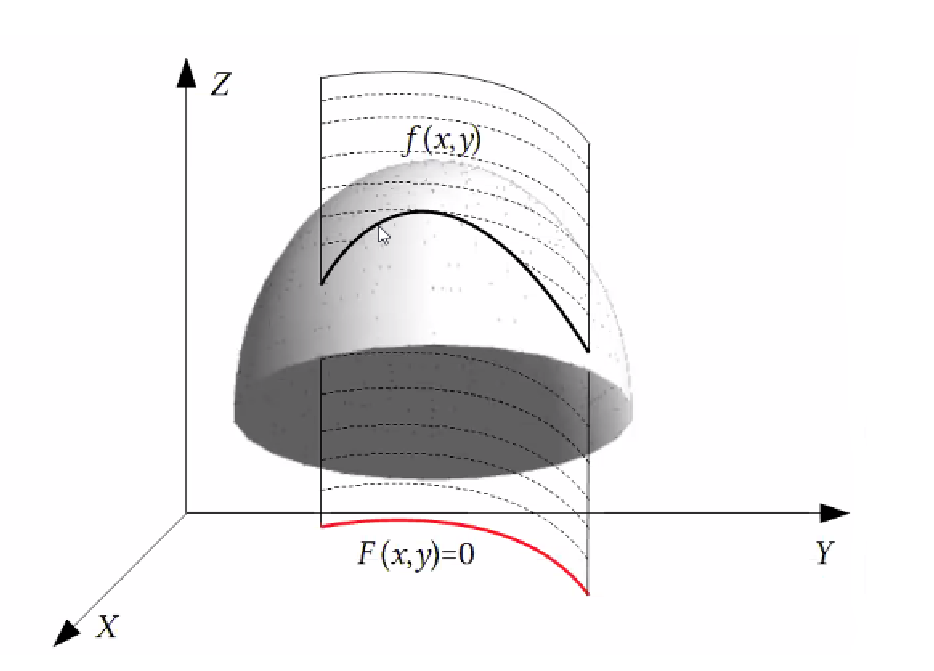
\includegraphics[scale=0.4]{img/rzut_plaszczyznaXY.png}
\end{center}

\begin{przyklad}

\[ f(x,y) = -xy, \ F(x,y) = 2x + y = 0 \]

\begin{center}To daje \ $ y = -2x $ \ czyli\end{center} 
\[ f(x,y) = f(x, -2x) = 2x^2, \ y=-2x, \ x\in \mathbb{R} \]

\begin{center}Czyli zbiór punktów\end{center}
\[ (x, -2x, 2x^2), \ x \in \mathbb{R} \]

Jest to paraboloida ustawiona "pionowo" ale nad prostą \ $ y= -2x $ \ (w płaszczyźnie równoległej do osi $Z$ i zawierającej tą prostą).

\begin{center}
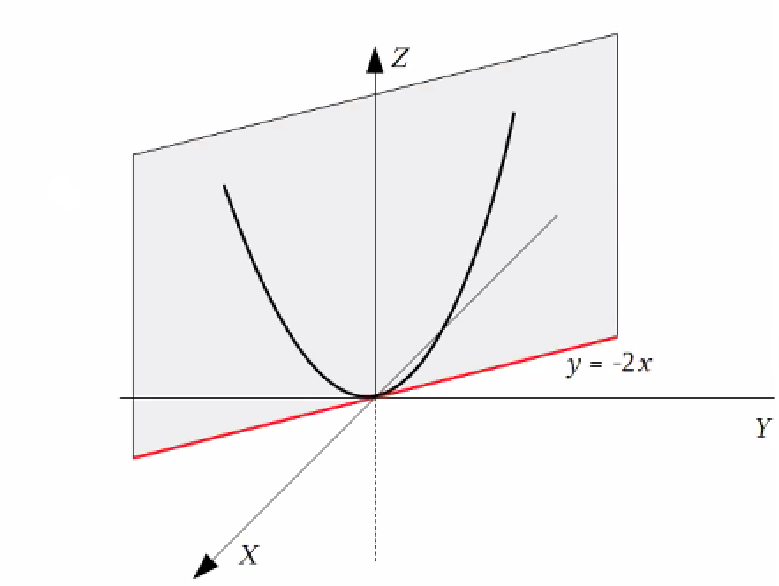
\includegraphics[scale=0.5]{img/paraboloida_przyklad.png}
\end{center}


Ekstrema warunkowe to ekstrema takich funkcji. Liczymy je metodami poznanymi z Analizy Matematycznej 1 (mamy funkcję 1 zmiennej).

W naszym przykładzie mamy do analizy funkcję \ $ f(x) = x^2, \ x \in \mathbb{R} $

Nie trzeba pochodnych, ekstremum to punkt dla \ $x = 0$ -- jest to minimum.

To daje \ $ y = -2 \cdot 0 = 0 $ \ oraz \ $ z = f(0,0) = 0 $ \ więc punkt $ (0,0,0) $.
\end{przyklad}

\subsection{Wartości największe i najmniejsze funkcji na zadanych zbiorach}

Mamy funkcję \ $ f(x,y), \ D_f = D $

Interesuje nas wartość największa i wartość najmniejsza $f$ na $D$. Te wartości mogą istnieć lub nie. To zależy od funkcji i zbioru.
\bigskip

\begin{tw}{Twierdzenie (Wersja tw. Weiertrassa (AM1) dla funkcji dwóch zmiennych)}

Gdy $D$ jest domknięty (czyli cały brzeg $D$ jest zawarty w $D$) oraz ograniczony (czyli zawiera się w pewnym kole) i $f$ jest ciągła
na $D$ to wartość największa i wartość najmniejsza $f$ na $D$ są osiągane.
\end{tw}
\bigskip

Gdzie te wartości mogą być osiągane dla funkcji różniczkowalnych?
\begin{itemize}
    \item W punktach stacjonarnych $f$: $ f_x = f_y = 0 $.
    \item Na brzegu $D$: prowadzi to do funkcji warunkowych i ich wartości największych/najmniejszych -- jak dla funkcji jednej zmiennej w AM1
\end{itemize}
\bigskip

Dla punktów z obu przypadków liczymy wartości $f$ i z tych wartości wybieramy najwiekszą i najmniejszą. To daje odpowiedź.

\underline{Uwaga}: Dla punktów stacjonarnych \underline{nie trzeba sprawdzać czy jest to ekstremum}.

Nie potrzeba hesjanu itd. Wystarczy policzyć wartość.
\bigskip

\begin{przyklad}
\[ f(x,y) = xy^2, \ x^2 + y^3 \leq 3 \]

Punkty stacjonarne

$ f_x = y^2 = 0 $

$ f_y = 2xy = 0 $

Wychodzą punkty $ (x, 0) $ oraz $ f(x,0) = \textcolor{magenta}{0} $

Brzeg: \ $ x^2 + y^2 = 3 $. Wystarczy wyliczyć \ $ y^2 = 3 - x^2 $ \ i to daje
\[f(x,y) = f(x) = x(3-x^2) = 3x - x^3, \ x\in \left[-\sqrt3, \sqrt3 \right] \]

Zadanie staje się zadaniem z AM1: znaleźć wartość największą/najmniejszą tej funkcji.

Zatem

\[ f(\pm \sqrt3) = \textcolor{magenta}{0} \]
\[ f' = 3 - 3x^2 = 0 \ \Leftrightarrow \ x = \pm 1 \in \left[ -\sqrt3, \sqrt3 \right] \]
\[ f(-1) = \textcolor{magenta}{-2}, \ f(1) = \textcolor{magenta}{2} \]

Stąd wartość największa to 2, jest osiągana w punktach \ $(1, \sqrt2) $ \ oraz \ $ (1, -\sqrt2) $.

Najmniejsza wartość to -2, jest osiągana w punktach \ $(-1, \sqrt2) $ \ oraz \ $(-1, -\sqrt2) $.
\end{przyklad}


\subsection{Zadania optymalizacyjne}

Schemat taki jak w AM1.
\begin{enumerate}
    \item Ułożyć funkcję opisującą daną wielkość.
    \item Znaleźć dziedzinę tej funkcji pasującą do zadania (niekoniecznie dziedzinę naturalną).
    \item Znaleźć wartość największą lub najmniejszą tej funkcji na zadanej dziedzinie.
\end{enumerate}
\bigskip

\begin{przykladbig}

Spośród wszystkich trójkątów o obwodzie równym $3$ jednostki znaleźć ten trójkąt, który ma największe pole.
\medskip

1. Wzór funkcji.

Jeśli boki tego trójkąta mają długości $a,b,c > 0$ to pole jest dane wzorem
\[ S = \sqrt{p(p-a)(p-b)(p-c)} \textrm{ \ gdzie \ } p = \frac{a+b+c}{2} \quad \textrm{(wzór Herona)} \]
\medskip

2. Dziedzina $f$: $ a,b > 0, \ c = 3 - a - b > 0 $ \ oraz z warunku trójkąta

\[ \begin{array}{ccc} 
    a+b>c & \Leftrightarrow & b > 1,5 - a \\
    a+c>b & \Leftrightarrow & 0 < b < 1,5 \\
    b+c>a & \Leftrightarrow & 0 < a < 1,5
\end{array} \]

To daje trójkąt o wierzchołkach w punktach \ $(1.5, \ 0), (0, \ 1.5)$ oraz $(1.5, \ 1.5)$ \ ale bez brzegu.
Aby mieć gwarancję istnienia wartości największej (twierdzenie Weiertrassa) dołączamy brzeg do trójkąta i mamy $D_f$:

\[ 0 \leq a \leq 1,5 \]
\[ 1,5 - a \leq b \leq 1,5 \]

\begin{center}
    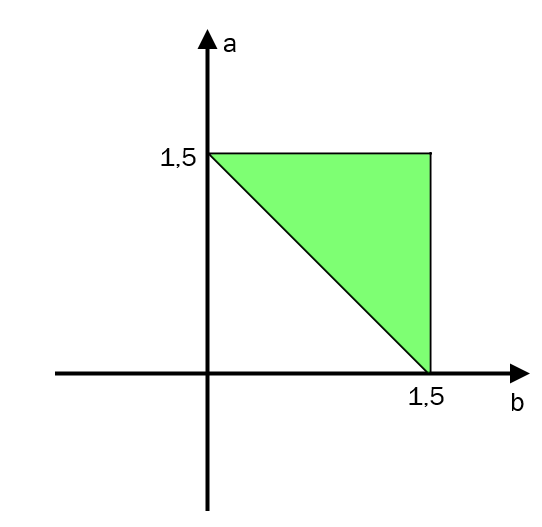
\includegraphics[scale=0.5]{img/trojkat.png}
\end{center}
\bigskip

3.Wartość największa $f$ \bigskip

a) Na brzegu

Brzeg składa się z trzech boków o równaniach
\[ \begin{array}{cc}
    a = 1,5: & f \equiv \textcolor{magenta}{0} \\
    b = 1,5: & f \equiv \textcolor{magenta}{0} \\
    b = 1,5 - a: & f \equiv \textcolor{magenta}{0} \\
\end{array}
\]

To na pewno nie jest wartość największa \bigskip

b) W punktach stacjonarnych we wnętrzu

\[ f(a,b) = \sqrt{1,5(1,5-a)(1,5-b)(a+b-1,5)} \quad \textrm{więc} \]
\[ f_a = \frac{1}{2\sqrt{do poprawy}} \cdot 1,5 \cdot (1,5 - b) \cdot (-(a+b - 1,5) + 1(1,5 - a)) = 0 \]

To daje układ

\[ \begin{cases} (1,5 - b) \cdot (3 - 2a - b) = 0 \\ (1,5 - a) \cdot (3 - 2b - a) = 0 \end{cases} \]

Zatem 

\[ \begin{cases} b = 1,5 \ \textrm{brzeg -- odrzucamy} \ \lor \ 3 - 2a - b = 0 \\
    a = 1,5 \ \textrm{brzeg -- odrzucamy} \ \lor \ 3 - 2b - a = 0
\end{cases} \]

Dla punktów we wnętrzu trójkąta jest więc

\[ 
\begin{cases}
    3 - 2a - b = 0 \\
    3 - 2b - a = 0
\end{cases}    
\]

To daje \ $ a = b = 1$ oraz \ $ f(1,1) = \textcolor{magenta}{\frac{\sqrt3}{4}} $. To jest wartość największa.

Ponadto wtedy $c = 1$. Jest to więc trójkąt równoboczny.
\end{przykladbig}

\end{document}